\documentclass[a4paper]{article}
\usepackage{graphicx} % Required for inserting images
\graphicspath{{./images/}}


%% Language and font encodings
\usepackage[english]{babel}
\usepackage[utf8x]{inputenc}
\usepackage[T1]{fontenc}
\usepackage{booktabs}
\usepackage{algorithm}
\usepackage{algorithmicx}
\usepackage{amsfonts}
\usepackage{algpseudocode}
\usepackage{color,soul}
\usepackage{multicol}
\usepackage{amsmath}
\usepackage{amssymb}
\usepackage{wrapfig}
\usepackage{hyperref}
\usepackage{tikz}  %
\usetikzlibrary{positioning}
\usepackage{subcaption}
\usepackage{xcolor}
\usepackage{stmaryrd}





\usepackage{courier} %% Sets font for listing as Courier.
\usepackage{listings, xcolor}
\lstset{
tabsize = 4, %% set tab space width
showstringspaces = false, %% prevent space marking in strings, string is defined as the text that is generally printed directly to the console
numbers = left, %% display line numbers on the left
commentstyle = \color{orange}, %% set comment color
keywordstyle = \color{blue}, %% set keyword color
stringstyle = \color{red}, %% set string color
rulecolor = \color{black}, %% set frame color to avoid being affected by text color
basicstyle = \small \ttfamily , %% set listing font and size
breaklines = true, %% enable line breaking
numberstyle = \tiny,
}

%%damit I.H über = steht
\newcommand\myEqualOne{\mathrel{\overset{\makebox[0pt]{\mbox{\normalfont\tiny\sffamily I.H}}}{=}}}


%% Sets page size and margins
\usepackage[a4paper,top=3cm,bottom=2cm,left=3cm,right=3cm,
            marginparwidth=1.75cm]{geometry}

%%--------------------------begin Document--------------------------------
\title{Algorithmen und Datenstrukturen 2023}
\author{bergery@student.ethz.ch}
\date{Oktober 2023}

\begin{document}
\maketitle
\begin{center}
    
\includegraphics{Pictures/eth_logo_kurz_pos Kopie.png}
\end{center}

\tableofcontents
\newpage

%%Chapter 01
\section{Vorwort}
Dieses Skript dient dazu eine grobe Übersicht für die Vorlesung "Algorithmen und Datenstrukturen" zu geben. Jegliche Informationen dieses Skriptes sollte man an der Prüfung können.\\
Für Fehler in diesem Skript wird keine Verantwortung übernommen.

%%Chapter 02
\section{Mathematische Grundlagen}
\subsection{Induktion}
    Die vollständige Induktion ist eine mathematische Beweismethode, nach der eine Aussage für alle natürlichen Zahlen bewiesen wird, die größer oder gleich einem bestimmten Startwert sind. Da es sich um unendlich viele Zahlen handelt, kann eine Herleitung nicht für jede Zahl einzeln erbracht werden. Sie ist ein deduktives Verfahren. \\
    Der Beweis, dass die Aussage $A(n)$ für alle $n \geq n_0 (n_0$ meist 0 oder 1), gilt, wird dabei in zwei Etappen durchgeführt:
    \begin{enumerate}
        \item Im \textit{Induktionsanfang} wird die Gültigkeit der Aussage $A(n_0)$ für eine kleinste Zahl $n_0$ gezeigt.
        \item Im \textit{Induktionsanfang} wird für ein beliebiges $n \geq n_0$ die Gültigkeit der Aussage $A(n+1)$ aus der Gültigkeit von $A(n)$ geschlussfolgert.
    \end{enumerate}
    \textbf{Beispiel:} \\
        Aussage: $A(n):= 1 + 2 + 3 + ...+ n = \frac{n \cdot (n+1)}{2}$ für $n \geq 1$ \\
        \textit{Base Case}: Für $n = 1$ gilt: $1 = \frac{1 \cdot (1+1)}{2} \rightarrow 1 = 1 \ \checkmark$ \\
        \textit{Induction hypothesis}: "We now assume that it is true for $n = k$, i.e., $1 + 2 + 3 + ...+ k = \frac{k \cdot (k+1)}{2} $.
        \textit{Induction step}: $k \rightarrow k+1$ \\
        $1 + 2 + 3 + ...+ k + (k+1) \myEqualOne  \frac{k \cdot (k+1)}{2} + (k+1)$, where $\frac{k \cdot (k+1)}{2} + (k+1) = \frac{k^2 + 3k + 2}{2} = \frac{(k+1) \cdot (k+2)}{2} \ \square.$
        By the principle of mathematical induction, we conclude that $ 1 + 2 + 3 + ...+ n = \frac{n \cdot (n+1)}{2}$ is true for all $n \in \mathbb{N}.$
        \\
        
    \subsection{Wichtige Annäherungen}
    Damit wir schnelle Resultate erhalten können, sind Approximationen ein fundamentaler Bestandteil. Aus diesem Grund folgende Liste:

    \begin{itemize}
        \item  $n! \leq n^n, $ for $  n\geq 1 $
        \item $\big(\frac{n}{2}\big)^{{n}/{2}} \leq n!, \ for\ n\geq 1 $
        \item $ \sum_{i=0}^{n} \log n  = \ \log\prod_{i=1}^{n}n = \log{n!} \ \approx n\log n \to\mathcal{O}(n \log n)$
        \item $\sum_{i=0}^{n} 1 = (n+1)  \to \mathcal{O}(n)$
        \item $\sum_{i=0}^{n} i = \frac{n(n+1)}{2} \to \mathcal{O}(n^2)$
        \item $\sum_{i=0}^{n} i^2 = \frac{n(n+1)(2n+1)}{6} \to \mathcal{O}(n^3)$
        \item $\sum_{i=0}^{n} i^3 = \frac{n^2(n+1)^2}{4}  \to\mathcal{O}(n^4)$
        \item binomial coefficient: $\binom{n}{k}= \frac{n!}{k!(n-k)!}$
        \item $\binom{n}{0}=\binom{n}{n}=1  \quad\quad
              \binom{n+1}{k+1}=\binom{n}{k}+\binom{n}{k+1}  \quad\quad
              \binom{n}{n-k}=\binom{n}{k}$
        \item $\sum_{i=1}^{n}i^k \leq \sum_{i=1}^{n}n^k$
    \end{itemize}
        

    \subsection{Big-O Notation}
    Landau-Symbole (engl. Big-O notation) werden verwendet, um das asymptotische Verhalten von Funktionen und Folgen zu beschreiben.
    In der Informatik werden sie bei der Analyse von Algorithmen verwendet und geben ein Maß für die Anzahl der Elementarschritte oder der Speichereinheiten in Abhängigkeit von der Größe des gegebenen Problems an. \\
    Für Annäherungen wird auch sehr oft die \textbf{Regel von de l'Hôpital} \label{Hôpital} angewendet:\\
        Let $f, g : \mathbb{R}\to\mathbb{R}$ be differentiable functions with $f(x)\to\infty, g(x)\to\infty$ for $x\to\infty$. \\
        If $\lim_{x\to\infty}\frac{f'(x)}{g'(x)}$ exists, then
        $\lim_{x\to\infty}\frac{f(x)}{g(x)}=\lim_{x\to\infty}\frac{f'(x)}{g'(x)}$


    

    \subsubsection{Definition O-Notation}
    In der Tabelle (\ref{tab:ONotation}) sehen wir jegliche Definition der $\mathcal{O}$-Notation.
    Wir unterscheiden zwischen, $\Omega$ (Omega) [lower-bound], $\Theta$ (Theta) [tight-bound] und  $\mathcal{O}$ [upper-bound]. Damit dies noch mathematisch formuliert ist haben wird folgendes: \\
    Let $f, g: \mathbb{R} \rightarrow \mathbb{R}^+$ such that the limit of $\frac f g$ exists. Then:
    
    \begin{equation*}
    \lim_{x\to\infty}\frac fg = \infty \Rightarrow g \in \mathcal{O}(f) \text{ and } f \in \Omega(g)
    \end{equation*}
    \begin{equation*}
    \lim_{x \rightarrow \infty} \frac fg = C \in \mathbb{R}^+ \setminus \left\lbrace 0 \right\rbrace \Rightarrow f \in\Theta(g)  \text{ and } g \in\Theta(f) \\
    \end{equation*}
    \begin{equation*}
    \lim_{x \rightarrow \infty} \frac fg = 0 \Rightarrow f \in\mathcal{O}(g) \text{ and } g \in\Omega(f) \\
    \end{equation*}
    
    \subsubsection{*Upper bound (big-O)}
    $$\mathcal{O}(g) :=\lbrace f: \mathbb{N}\to\mathbb{R}^+\mid\exists c\in\mathbb{R}^+, n_0\in\mathbb{N}, \forall n\geq n_0 : f(n)\leq c\cdot g(n)\rbrace$$
    
    $$\mathcal{O}(f) \leq O(g) \Leftrightarrow \exists c, n_0 . \forall n \geq n_0 . f(n) \leq c\cdot g(n)  $$
    
    \subsubsection*{Lower bound (big-Omega)}
    $$\Omega(g) :=\lbrace f: \mathbb{N}\to\mathbb{R}^+\mid\exists c\in\mathbb{R}^+, n_0\in\mathbb{N}, \forall n\geq n_0 : f(n)\geq c\cdot g(n)\rbrace$$
    
    $$\Omega(f) \geq \Omega(g) \Leftrightarrow \exists c, n_0 . \forall n \geq n_0 . f(n) \geq c\cdot g(n)  $$
    
    \subsubsection*{Tight bound (big-Theta)}
    $$\Theta(g) :=\lbrace f: \mathbb{N}\to\mathbb{R}^+\mid\exists c_1, c_2\in\mathbb{R}^+, n_0\in\mathbb{N}, \forall n\geq n_0 : 0 \leq c_1 g(n)\leq f(n)\leq c_2 g(n)\rbrace$$
    
    $$\Theta(f) = \Theta(g) \Leftrightarrow \exists c_1, c_2 n_1, n_2 . \forall n \geq n_1 . f(n) \leq c\cdot g(n) \land \forall n \geq n_2 . f(n) \geq c\cdot g(n)  $$
    Therefore: 
    $$\Theta(f) = \Theta(g) \Leftrightarrow O(f) \leq O(g) \text{ and } \Omega(f) \geq \Omega(g)$$
    
    
    \textbf{Wichtiger Hinweis:} Implikationspfeil anschauen: $\mathcal{O}(f) \implies \lim_{x\to\infty}\frac fg = \infty \ \lightning$
    
    


    \begin{table}
        \centering
        \small
        \begin{tabular}{c|c|c}
            Notation & Definition & Mathematische Definition \\
            \hline
            $f \in o(g)$ 
            & asymptotisch gegenüber $g$ vernachlässigbar 
            & $\lim_{x\to a} \big| \frac{f(x)}{g(x)} \big| = 0 $\\
            
             $f \in \mathcal{O}(g)$
             & asymptotische obere Schranke  
             & $\limsup_{x\to a} \big| \frac{f(x)}{g(x)} \big| < \infty $ \\
             
            $f = \Omega(g)$ 
            & asymptotische untere Schranke, $f$ ist nicht in $o(g)$ 
            & 
            $\limsup_{x\to a} \big| \frac{f(x)}{g(x)} \big| > 0 $\\

            $f \in \Theta(g)$            
            & scharfe Schranke,  sowohl $f \in \mathcal{O}(g)$ als auch $f \in \Omega(g)$
            &  $0 < \liminf_{x\to a} \big| \frac{f(x)}{g(x)} \big| \leq \limsup \big| \frac{f(x)}{g(x)} \big| < \infty $ \\

            $f \in \omega(g)$
            &  asymptotisch dominant, $g \in o(f)$
            & $\lim_{x \to a}\frac{f(x)}{g(x)} \big| = \infty$ \\
        \hline
        \end{tabular}
        \caption{Definition der $\mathcal{O}$-Notation}
        \label{tab:ONotation}
    \end{table}
    
    \subsubsection{Master Theorem}
    Damit das Rechnen mit solchen Grenzwerten schneller geht, haben wir das Master-Theorem, welches sehr praktische Anwendung mit sich bringt:
      \begin{equation} \label{MasterTheorem}
  T(n) \leq aT(n/2)\ + Cn^b: =\begin{cases}      T(n) \leq \mathcal{O}(n^b), & \text{b >} \log_2(a)\\
      T(n) \leq \mathcal{O}(n^b\log(n)) &\text{b =} \log_2(a)\\
      T(n) \leq \mathcal{O}(n^{\log_2(a)}) & \text{b <} \log_2(a)
    \end{cases}         
  \end{equation}

    \subsubsection{Overview}
    Damit wir nun einmal sehen können wie die asympotischen Grenzen sich verhalten, folgende Abbildung: 
    \begin{figure}[h]
        \centering
        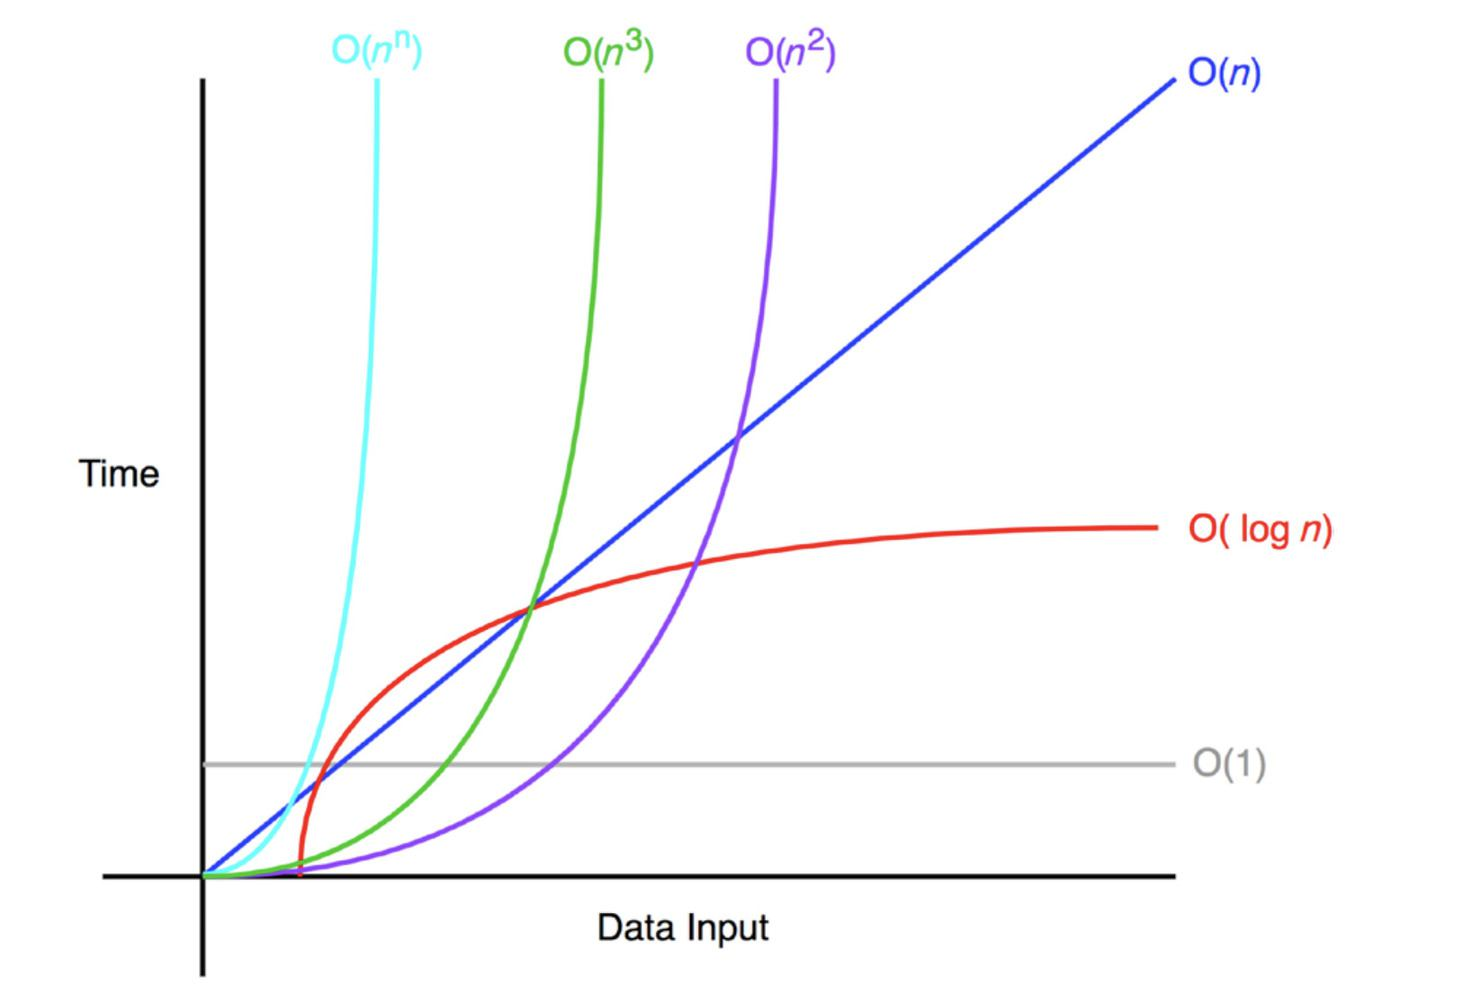
\includegraphics[width=0.3\textwidth]{Pictures/big-o-notation.jpg}
        \caption{Wachstum verschiedener Funktionen}
        \label{fig: WachstumBigO}
    \end{figure}
    Die graphische Darstellung der Funktionen im Bild (\ref{fig: WachstumBigO}) zeigt uns leider nur sechs Funktionen. 
    Um möglichst viele Funktionen in aufsteigendem, asymptotischen Wachstum zu sehen, folgende Abbildung:

    $\mathcal{O}(1) \in [\mathcal{O}(\frac{1}{n^2}) \in \mathcal{O}(\frac{1}{n}) \in \ ] \  \mathcal{O}(\log \log n)\in \mathcal{O}(\log n) \in \mathcal{O}(\sqrt{n}) \in \mathcal{O}(n) \in \mathcal{O}(n\log n) \in [\mathcal{O}({n^c}) \in \mathcal{O}(c^n) \in \ ] \mathcal{O}(n^2) \in \mathcal{O}(2^n) \in \mathcal{O}(2^{n^{2}}) \in \mathcal{O}(n!) $

\newpage
\subsection{Erster Algorithmus}
    \subsubsection{Maximum Subarray Sum}
    Für einen ersten Algorithmus schauen wir den \texttt{Maximum Subarray Sum} Algorithmus an. Dieser Algorithmus enthält ein Array von $n$ rationalen Zahlen $a_1,..., a_n$ und gesucht ist ein Teilstück mit maximaler Summe.  \\
    \textbf{Beispiel}: \\
    Sei ein Array [-2, -5, 6, -2, -3, 1, 5, -6] gegeben, so ist die maximale Teilsumme dieses Array 7, nämlich $ 6 + (-2) + (-3) + 1 + 5 = 7$. \\
      
\begin{algorithm}
    \caption{Maximum Subarray Sum $(a_1,..., a_n)$}
    \label{alg:MSS-1}
    \begin{algorithmic}[1]
    \Function{FindMSS}{Array [$1...n$]}
    \State $S_0 \gets 0$ 
    \For{$i \gets 1,...,n$}
        \State $S_i \gets S_{i-1} + a_i$ 
    \EndFor
    \State maxS $\gets 0$
    \For{$i \gets 1,...,n$}
        \For{$j \gets 1,...,n$}
            \State $S \gets S_j - S_{j-1}$ 
           \State Merke maximales S
        \EndFor
    \EndFor
    \EndFunction

    \end{algorithmic}
    
\end{algorithm}

Dieser naive Algorithmus führt insgesamt $\Theta(n^3)$ viele Additionen aus, was sehr schlecht ist für unseren Algorithmus.

\begin{algorithm}
 \caption{MSS divide and conquer $(a_1,..., a_n)$}
 \label{alg:MSS-Div}
 \begin{algorithmic}[1]
    \Function{MSSDivAndConquer}{Array [$1,...,n$]}
      \State Wenn $n=1$ ist, dann gib $max{a_1,0}$ zurück.
      \State Wenn $n>1$ ist:
      \State Teile die Eingabe in $A_1 = \langle a_1,...,a_{n/2} \rangle$ und $A_2 = \langle a_{n/2+1},...,a_{n} \rangle$ auf
      \State Berechne rekursiv den Wert $W_1$ einer besten Lösung für das Array $A_1$
      \State Berechne rekursiv den Wert $W_2$ einer besten Lösung für das Array $A_2$
      \State Berechne grösste Suffixsumme $S$ in $A_1$
      \State Berechne grösste Suffixsumme $P$ in $A_2$
      \State Setzte $W_3 \gets S+P$
      \State Gib max$\{W_1, W_2, W_3\}$ zurück
    \EndFunction
 \end{algorithmic}
\end{algorithm}

    Wir haben schon eine Verbesserung des Algorithmus von $\Theta(n^3)$ vielen Additionen zu $\Theta(n\log n)$ vielen Additionen. In einem letzten Schritt können wir diesen sogar noch einmal verbessern nämlich bis zu $\Theta(n)$ viele Additionen.

\begin{algorithm}
 \caption{MSS-Induktiv $(a_1,..., a_n)$}
 \label{alg:MSS-Induktiv}
    \begin{algorithmic}[1]
    \Function{MSSInduktiv}{Array [$1,...,n$]}
    \State $randmax \gets 0$
    \State $maxS \gets 0$
        \For{$i \gets 1,...,n$}
            \State $randmax \gets randmax + a_i$
            \If{$randmax > maxS$}
                \State $maxS \gets randmax$
            \EndIf
            \If{$randmax < 0$}
                \State $randmax \gets 0$
            \EndIf
        \State Gib $maxS$ zurück
        \EndFor
    \EndFunction
    \end{algorithmic}
\end{algorithm}

\newpage
%%Chapter 03
\section{Suchen und Sortieren}
\subsection{Suchen}
    In diesem Abschnitt schauen wir wie schnell wir in abstrakten Daten Strukturen suchen, einfügen und löschen können. Die meist gebrauchten Datenstrukturen sind somit in folgender Tabelle aufgeführt mit ihrer korrespondierender Laufzeit: \\
\begin{center}      
\begin{tabular} {|c|c|c|c|}
  \hline
  \label{Tab: LaufzeitenSuchSortier}
  \bfseries Data structure & \bfseries Search & \bfseries Insert & \bfseries Delete\\
  \hline
  Unsorted Array	&$O(n)$				&$O(1)$			&$O(n)$\\
  Sorted Array		&$O(\log{n})$	          	&$O(n)$			&$O(n)$\\
  Unsorted List 	&$O(n)$				&$O(1)$			&$O(n)$\\	
  Sorted List		&$O(n)$				&$O(n)$			&$O(n)$\\	
  Unbalanced Tree	&$O(n)$				&$O(n)$			&$O(n)$\\
  AVL tree		&$O(\log{n})$	        	&$O(\log{n})$	        &$O(\log{n})$\\
  \hline
\end{tabular}
\end{center}  
Wir stellen fest, dass es im Allgemeinen einen Kompromiss gibt zwischen einfachen Datenstrukturen, die ein einfaches Einfügen und Löschen ermöglichen, aber die Einträge nicht vorverarbeiten, um spätere Suchvorgänge zu erleichtern (ungeordnetes Array), und komplexeren Datenstrukturen mit höheren Einfüge- und Löschkosten, die effizienter abgefragt werden können.

\subsubsection{Binary Search} \label{BinarySearch}
    Binary Search ist der standart Suchalgorithmus für \textbf{sortierte} Arrays, da es einen effizienten, logarithmische Laufzeitkomplexität hat.

\begin{algorithm}
\caption{Binary search} 
\label{alg:BinarySearch}
\begin{algorithmic}[1] 
  \Function{FindIndex}{$A$, $e$} \Comment{Search item $e$ in sorted array $A$}
  \State $l, r \gets 0, A\texttt{.length}-1$
  \While{$r > l$}
  \State $m \gets \left\lfloor \frac{l+r}{2} \right\rfloor$
  \If{$A\left[m\right] = e$}
  \State \Return $m$
  \ElsIf{$A\left[m\right] > e$}
  \State $r \gets m-1$
  \Else
  \State $l \gets m+1$
  \EndIf
  \EndWhile
  \State \Return \texttt{"not found"}
  \EndFunction
\end{algorithmic}
\end{algorithm}
Obwohl bei der binären Suche die Kosten für die Suche in geordneten Arrays logarithmisch werden, sind Einfügung und Löschung immer noch linear: im schlimmsten Fall, d.h. wenn das einzufügende oder zu löschende Element das erste Element des Arrays ist, müssen wir alle Elemente um einen Schritt nach rechts/links verschieben.

\subsubsection{Heaps}
Noch effizienter als geordnete Arrays sind daher baumartige Strukturen, bei denen die Kosten für das Einfügen und Löschen ebenfalls logarithmisch sein können. Heaps sind eine spezielle Klasse von baumbasierten Strukturen, die eine effiziente (zeitkonstante) Methode zur Extraktion des kleinsten oder größten Elements bieten.

Genauer gesagt sind Min- (bzw. Max-) Heaps baumbasierte Datenstrukturen, die die folgende Heap-Invariante erfüllen: Wenn $A$ das Elternteil von $B$ ist, dann ist der Wert von Knoten $A$ kleiner (bzw. größer) als der Wert von Knoten $B$. Wir betrachten hier binäre Min-Heaps, was bedeutet, dass ein Elternteil einen kleineren Wert hat als seine (höchstens zwei) Kinder. Für binäre Min-Haufen gilt zusätzlich die folgende Forminvariante: Der betrachtete Haufen ist immer ein vollständiger binärer Baum, d. h. alle Schichten des Baums sind von oben nach unten und von links nach rechts gefüllt.


\begin{figure}[h] 
\caption{Beispiel eines Min-Heaps}
\centering
\label{fig: Min-heap}
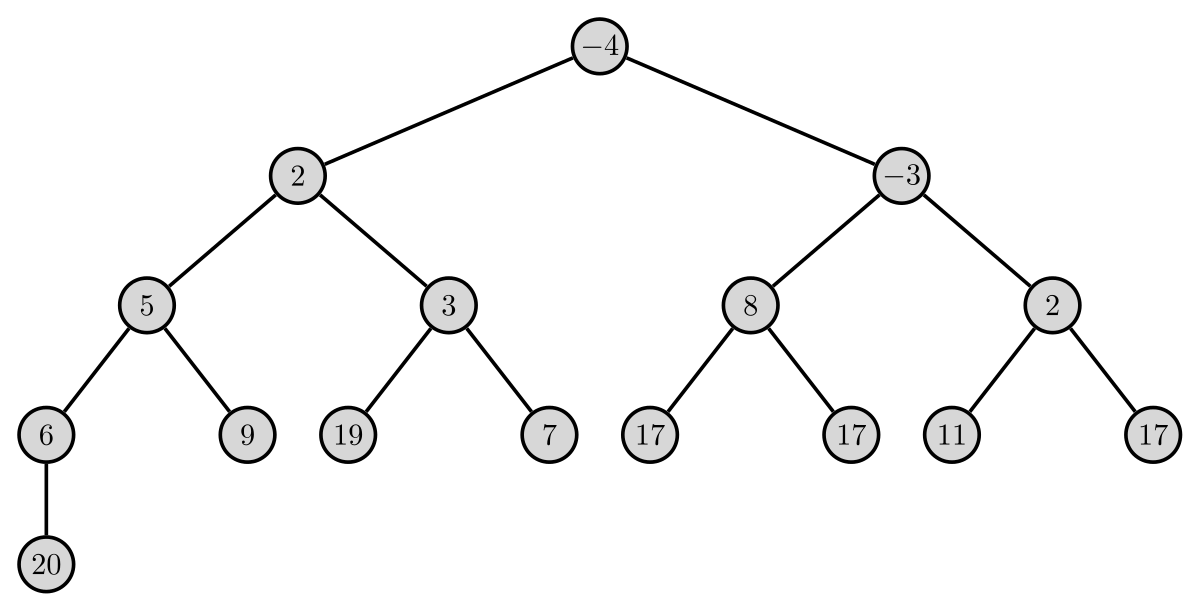
\includegraphics[scale= 0.2]{Pictures/Heap.svg.png}
\end{figure}

\begin{figure}[h] 
\caption{Beispiel 0-Heaps}
\centering
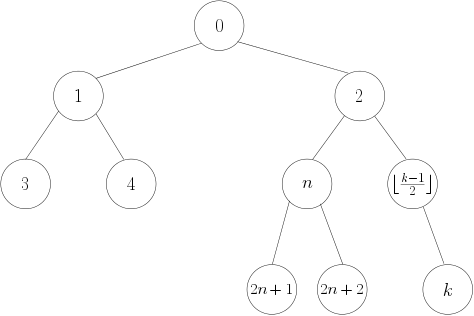
\includegraphics[scale= 0.5]{Pictures/0-heap.png}
\label{fig: 0-Heap}
\end{figure}



\subsubsection*{Implementation}
Die gebräuchlichste Implementierung ist ein Array (mit fester oder dynamischer Größe). Geht man von einem 0-basierten Array aus (vgl. Figure \ref{fig: 0-Heap}), so sind die \textit{children} des Knotens $n$, $2n+1$ und $2n+2$ und die \textit{parent} des Knotens $k$ ist der Knoten $\lfloor \frac{k-1}{2}\rfloor$.

\newpage
\subsubsection*{Common operations} \label{common operations}
Here are the most common operations that a min-heap must support:
\begin{itemize}
\item \textbf{Basic operations}
  \begin{itemize}
  \item Find min,
  \item Delete min,
  \item Insert,
  \item Find min and delete it (pop);
  \end{itemize}
\item \textbf{Initialization}
  \begin{itemize}
  \item Create empty heap,
  \item Heapify (transform array into heap);
  \end{itemize}
\item\textbf{Inspection}
  \begin{itemize}
  \item Return size,
  \item Test if empty;
  \end{itemize}
\item \textbf{Other}
  \begin{itemize}
  \item Increase/decrease,
  \item Delete,
  \item Restore heap invariant,
  \item Merge/union.
  \end{itemize}
\end{itemize}


\subsubsection*{Preserving the heap invariant}
Die Heap Invariante sagt uns eigentlich aus: 
\begin{quote}
    "Das Label jedes Knoten $n$ ist kleiner oder gleich den Labels der Kinder von $n$."
\end{quote}
Bei der Aktualisierung eines Heaps ist es wichtig, die oben beschriebene Invariante beizubehalten. Nach einer Löschung oder einer Einfügung kann es vorkommen, dass ein (einzelnes) Element kleiner wird als eines seiner Kinder; wir können dann die Heap-Invariante in logarithmischer Zeit wiederherstellen, indem wir dieses Element nach unten durchsickern lassen. (Vgl. Durchsickeralgorithmus \ref{alg:DurchsickernHeap})

\begin{algorithm}
\caption{Restore heap invariant by percolating element down} 
\label{alg:DurchsickernHeap}
\begin{algorithmic}[1] 
  \Function{PercolateDown}{$H$, $i$} \Comment{Percolate element $i$ in $H$}
  \State $e \gets H\left[i\right]$
  \If{$2i+2 = H\texttt{.length}$}
  \If{$e > H\left[2i+1\right]$}
  \State Swap $H\left[i\right]$ and $H\left[2i+1\right]$
  \EndIf
  \ElsIf{$2i+2 < H\texttt{.length}$}
  \State $l, r \gets H\left[2i+1\right], H\left[2i+2\right]$
  \If{$l < r$}
  \If{$l < e$}
  \State Swap $H\left[i\right]$ and $H\left[2i+1\right]$
  \State \textsc{PercolateDown}$\left(H, 2i+1\right)$
  \EndIf
  \Else
  \If{$r < e$}
  \State Swap $H\left[i\right]$ and $H\left[2i+2\right]$
  \State \textsc{PercolateDown}$\left(H, 2i+2\right)$
  \EndIf
  \EndIf
  \EndIf  
  \EndFunction
\end{algorithmic}
\end{algorithm}

\subsubsection*{Costs}

In der folgenden Tabelle sind die Kosten von Standard-Heap-Operationen für drei Arten von Heaps zusammengefasst: binäre Heaps, binomische Heaps und Fibonacci-Heaps. \\

\begin{tabular}{|c|c|c|c|}
  \hline
  \label{Tab: KostenHeaps}
\textbf{Operation}    & \textbf{Binary}             & \textbf{Binomial}         & \textbf{Fibonacci}   \\
\hline
search min   & $\Theta(1)$        & $\Theta(1)$      & $\Theta(1)$ \\
delete min   & $\Theta(\log n)$   & $\Theta(\log n)$ & $O(\log n)$ \\
insert       & $\Theta(\log n)$   & $\Theta(1)$      & $\Theta(1)$ \\
increase key & $\Theta(\log n)$   & $\Theta(\log n)$ & $\Theta(1)$ \\
  union        & $\Theta(m \log n)$ & $O(\log n)$      & $\Theta(1)$  \\
                                                         \hline
\end{tabular}


\subsubsection*{Zusammenfassung- Youtube}
\href{https://www.youtube.com/watch?v=0wPlzMU-k00}{Kurze Zusammenfassung anschauen}

\subsection{Binärer Suchbaum}
\subsubsection{Begrifflichkeiten}
Bäume im Allgemeinen gehören zu den wichtigsten in der Informatik auftretenden Datenstrukturen. Seien es Entscheidungsbäume, Syntaxbäume, Ableitungsbäume, Kodebäume oder auch Suchbäume. Bäume sind Listenstrukturen, ein Element referenziert einen \textbf{Knoten}. Jegliche Nachfahren die einen Knoten beinhalten nennt man \textbf{Kinder-Knoten}. Die \textbf{Wurzel} des Baumes ist, von welchem der Baum aus startet. Zusätzlich gilt, dass von jeder Wurzel der verschiedenen Knoten eines Baumes durch genau einen Pfad mit der Wurzel verbunden. Ein \textbf{Blatt} oder \textbf{Blätter} eines Baumes sind die Knoten welche keine Nachfolger haben. Im Beispiel von \ref{fig: binarytree} wären die Blätter dieses Baumes: [3, 7, 13, 18, 23]. Man nennt einen Baum \textbf{geordnet} wenn unter den Kinderknoten eines jeden Knotens eines Baumes eine \textbf{Anordnung definiert} ist, sodass man vom ersten, zweiten, dritten usw. Kinderknoten eines Knotens sprechen kann, so nennt man den Baum geordnet (Vgl. Figure \ref{fig: binarytree}). Im diesem Beispiel ist zu sehen, dass die definierte Anordnung wie folgt ist: Wenn der Wert eines Knotens kleiner ist als die Wurzel, so wird dieser links platziert, und dann wieder mit dem nächsten Knoten verglichen. Sofern dieser nun grösser ist, wie z.B Knoten 12, wird dieser rechts vom Knoten 5 platziert. \\
Ein weiterer Begriff, der wichtig ist im Kontext mit Bäumen ist die \textbf{Höhe} und \textbf{Tiefe} eines Baumes. Diese beiden Begriffe sind wie folgt definiert: 
\begin{itemize}
    \item $depth(v) = $ distance $v$ to root (along unique path)
    \item $height(T) = max_{v \in V} depth(v) + 1$
\end{itemize}
Man fasst die Knoten eines Baumes gleicher Tiefe zu \textbf{Niveaus} zusammen. Die Knoten auf dem Niveau $i$ sind alle Knoten der Tiefe $i$. Die Höhe des Beispiels (\ref{fig: binarytree}) wäre also der Pfad von $(15-5-12-10-6-7) + 1 = 6 $ und die Tiefe vom Knoten 20 wäre: 2. \\
Zusätzlich gilt: die Tiefe eines binary tree ist gleich wie die Höhe eines binary trees.\footnote{\href{https://www.baeldung.com/cs/binary-tree-height}{weitere Beispiele \& Erklärungen}}
Des weiteren heisst ein Baum \textbf{vollständig} wenn er auf jedem Niveau die maximal mögiche Knotenanzahl hat und sämtliche Blätter dieselbe Tiefe haben. 
Auch wie bei dem Heap gelten die "Basic operations": Einfügen, löschen, suchen eines Elementes und das Traversieren des Baumes (Vgl. \ref{common operations}).

\begin{figure}[h] 
\caption{Beispiel eines geordneten Binärbaumes}
\centering
\includegraphics[scale= 0.7]{Pictures/Pseudobinärersuchbaum.svg.png}
\label{fig: binarytree}
\end{figure}




\subsection{AVL-Trees}
Ein binärer Suchbaum ist \textit{AVL-ausgegelichen} oder höhenbalanciert. Kurz: Ein AVL Baum, wenn für jeden Knoten $p$ des Baumes gilt, dass sich die Höhe des linken Teilbaumes von der Höhe des rechten Teilbaumes von $p$ um höchstens 1 unterscheidet. In der folgenden Abbildung(\ref{fig: AVL-trees}) ist in (a)  und (c) ein AVL-Baum zu sehen. (b) hingegen ist kein AVL-Baum.\footnote{\href{https://www.cs.usfca.edu/~galles/visualization/AVLtree.html}{Animationen von AVL-Trees}}

\begin{figure}[h] 
\caption{Beispiel von zwei AVL-Bäume}
\centering
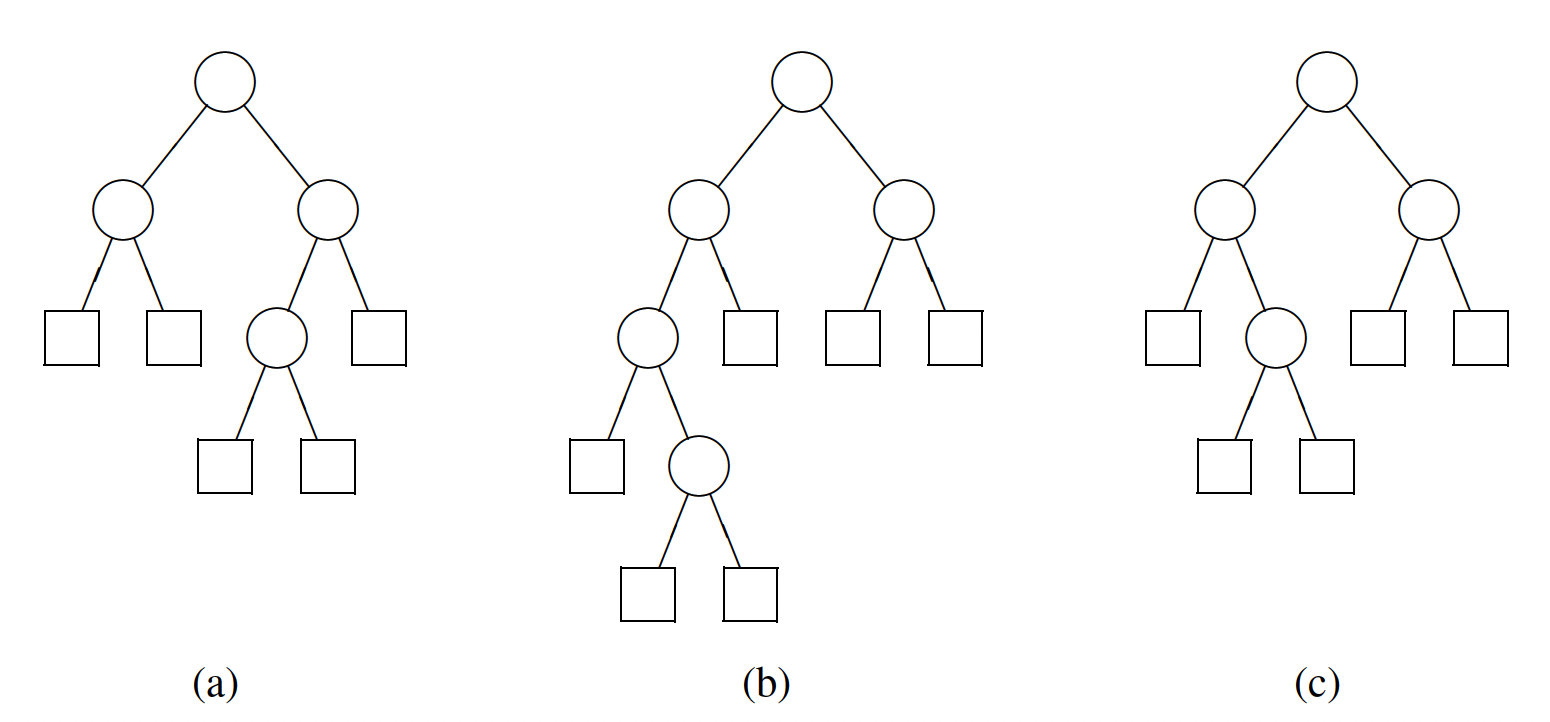
\includegraphics[scale= 0.5]{Pictures/AVL-trees.png}
\label{fig: AVL-trees}
\end{figure}

AVL-Bäume mit $N$ inneren Knoten und $N+1$ Blättern haben eine höhe von $\mathcal{O}(\log N)$. Man überlegt sich was die minimale Blatt-und Knotenzahl eines AVL-Baumes gegebener Höhe $h$ ist. Es gilt: AVL-Baum der Höhe 1 hat 2 Blätter und ein AVL-Baum der Höhe 2 mit minimaler Blattzahl hat 3 Blätter (Vgl. Figure \ref{fig: AVL-trees-height}). Ein AVL-Baum der Höhe $h+2$ mit minimaler Blattzahl erhält man, wenn man je einen AVL-Baum mit der Höhe $h+1$ und $h$ mit minimaler Blattzahl wie in Figure (\ref{fig: AVL-trees-allg}) zu einem Baum der Höhe $h+2$ zusammenfügt.

\begin{figure}[h] 
\caption{AVL-Baum mit Höhe 1 und 2}
\centering
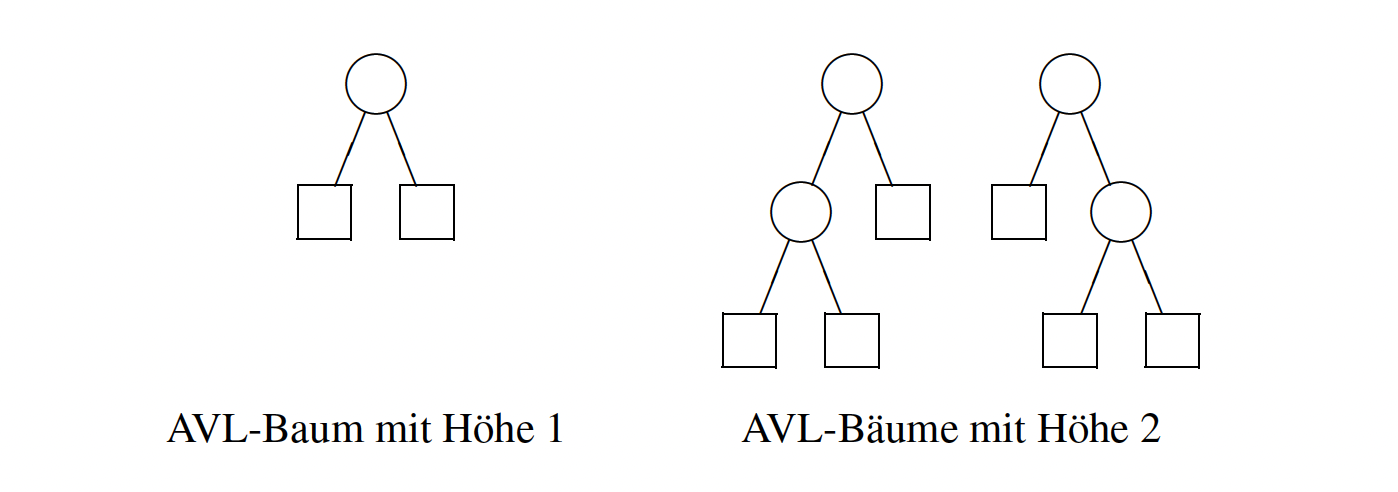
\includegraphics[scale= 0.5]{Pictures/AVL-trees-height.png}
\label{fig: AVL-trees-height}
\end{figure}

\begin{figure}[t] 
\caption{AVL-Baum }
\centering
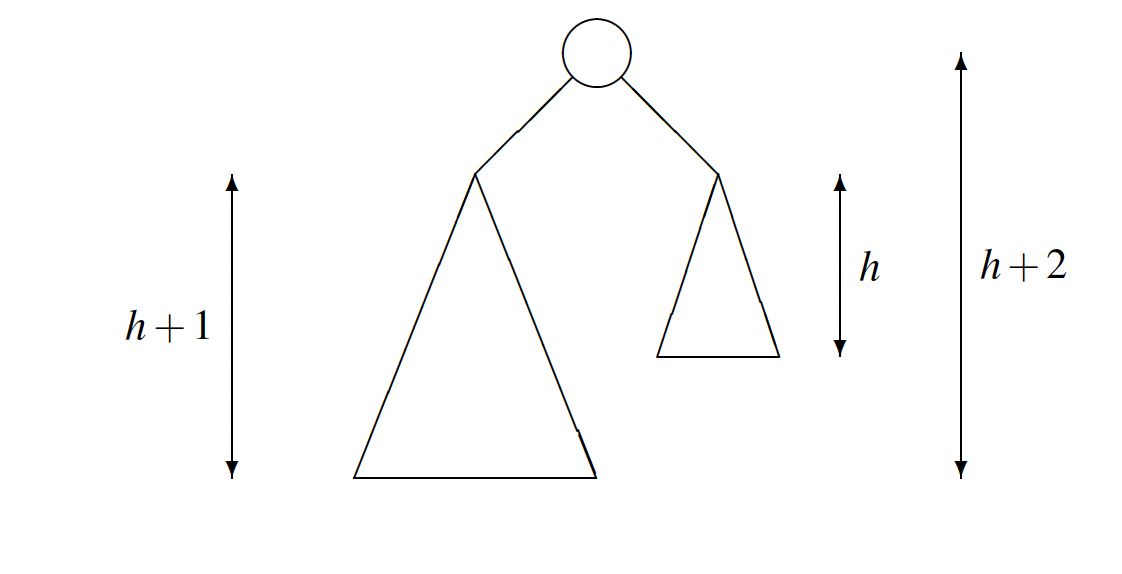
\includegraphics[scale= 0.5]{Pictures/AVL-trees-allg.png}
\label{fig: AVL-trees-allg}
\end{figure}

\newpage
\subsubsection{Suchen, Einfügen und Entfernen in AVL-Bäumen}
Da AVL-Bäume eigentlich binäre Suchbäume sind, kann man ihnen nach einem Schlüssel genauso suchen wie in einem natürlichen Baum. Im schlechtesten Fall ist die Suche nach einem Schlüssel von Wurzel bis zu einem Blatt. Da die Höhe logarithmisch beschränkt ist, wird dies im worst case $\mathcal{O} (\log N)$ Schritte benötigen, wobei der worst case in einem normalen binären Suchbaum $\mathcal{O} (N)$ ist (alle links oder rechts an der Wurzel). 

\subsubsection{Einfügen}\label{subsection EinfügenAVL}
Damit der Schlüssel eingefügt werden kann, überprüfen wir in einem ersten Schritt nach dem Schlüssel im Baum. Wenn dieser Schlüssel bereits vorhanden ist, endet der Vorgang. Sofern dieser aber nicht in dem Baum ist fügen wird diesen ein wie bei einem normalen Baum.

Das Problem welches wir nun erhalten ist die Aufrechterhaltung der AVL-Eigenschaft. Wenn wir bei Figure (\ref{fig: AVL-ausgangslage}) den Key 5 einfügen wollen, wird im nächsten Schritt Figure (\ref{fig:AVL-verletzt}) die Bedingung verletzt, da die Höhen des linken und rechten Teilbaumes sich um mehr als 1 unterscheiden. Man muss also die AVLAusgeglichenheit wieder herstellen. Dazu läuft man von der Einfügestelle den Suchpfad entlang zur Wurzel zurück und prüft an jedem Knoten (Vgl. \ref{eqn: bal(p)}, ob die Höhendifferenz  zwischen linkem und rechtem Teilbaum noch innerhalb der vorgeschriebenen Grenzen liegt. Ist das nicht der Fall, führt man eine so genannte Rotation oder eine Doppelrotation durch (Vgl. \ref{Rotationsabschnitt}), die die Sortierung der Schlüssel nicht beeinflusst, aber die Höhendifferenzen in den richtigen Bereich bringt.
\begin{figure}[h] 
   \centering
     \begin{subfigure}[h]{0.5\textwidth}
         \centering
         \includegraphics[scale = 0.3]{Pictures/AVL-einfügen1.png}
         \caption{Ausgangslage}
         \label{fig: AVL-ausgangslage}
     \end{subfigure}
     \hfill
     \begin{subfigure}[h]{0.45\textwidth}
         \centering
         \includegraphics[scale = 0.4]{Pictures/AVL.einfügen2.png}         \caption{AVL-Bedingung verletzt}
         \label{fig:AVL-verletzt}
     \end{subfigure}
     \caption{Wie die AVL-Eigenschaft verletzt werden kann}
    \label{fig: AVL-ausgangslage-verletzt}
\end{figure}

Man könnte vermuten, dass man zur Prüfung der Höhenbedingung an einem Knoten
im Baum die Höhen der Teilbäume des Knotens kennen muss. Das ist jedoch glücklicherweise nicht der Fall. Es genügt, an jedem inneren Knoten p den so genannten \textbf{Balancefaktor} $bal(p)$ mitzuführen, der wie folgt definiert ist:
\begin{equation} \label{eqn: bal(p)}
    bal(p) = \text{Höhe des rechten Teilbaumes von } p - \text{Höhe des linken Teilbaumes von } p
\end{equation}
\newpage
AVL-Bäume sind offenbar gerade dadurch charakterisiert, dass für jeden inneren Knoten $p$ gilt: $bal(p) \in \{ -1, 0, +1\}$. Um diese drei Fälle anzusehen, vergleichen wir diese in den folgenden Abbildungen \ref{fig: bal(p) für alle}:

\begin{figure}[h!]
\centering
\begin{subfigure}{0.6\textwidth}
    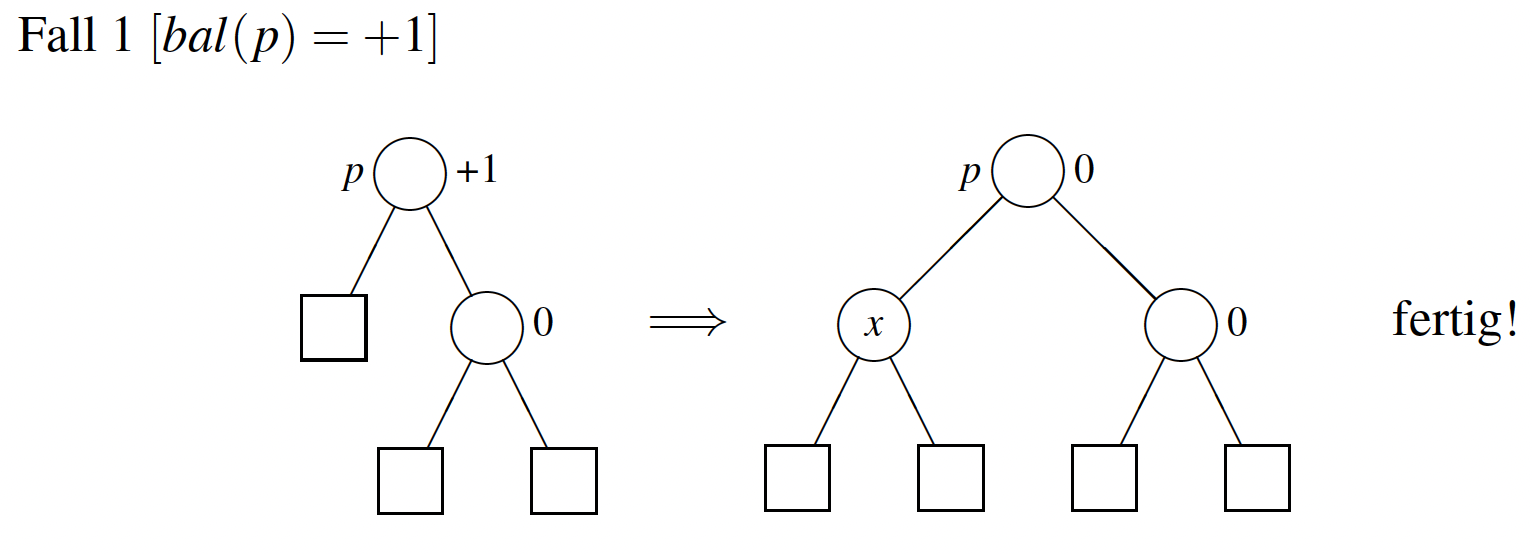
\includegraphics[width=\textwidth]{Pictures/AVL-bal(+1).png}
        \caption{$bal(p) = +1$}
        \label{fig: bal(p) = +1}
\end{subfigure}
\hfill
\begin{subfigure}{0.6\textwidth}
    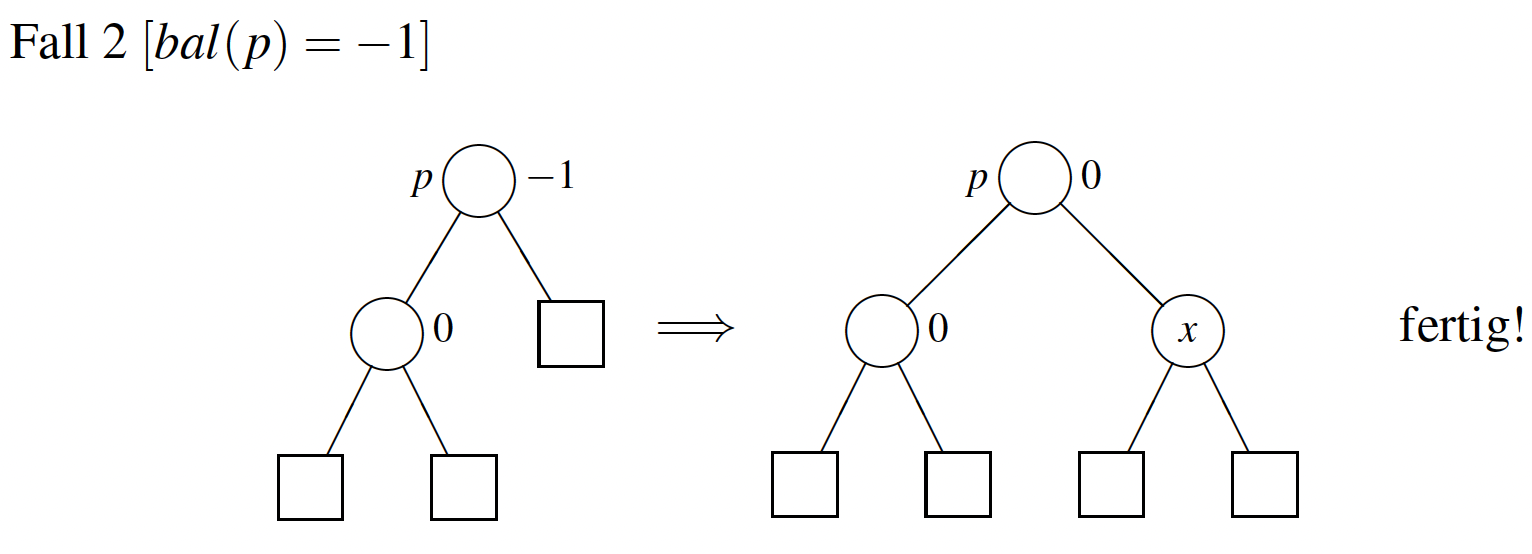
\includegraphics[width=\textwidth]{Pictures/AVL-bal(-1).png}
        \caption{$bal(p) = -1$}
        \label{fig: bal(p) = -1}
\end{subfigure}

\begin{subfigure}{0.6\textwidth}
    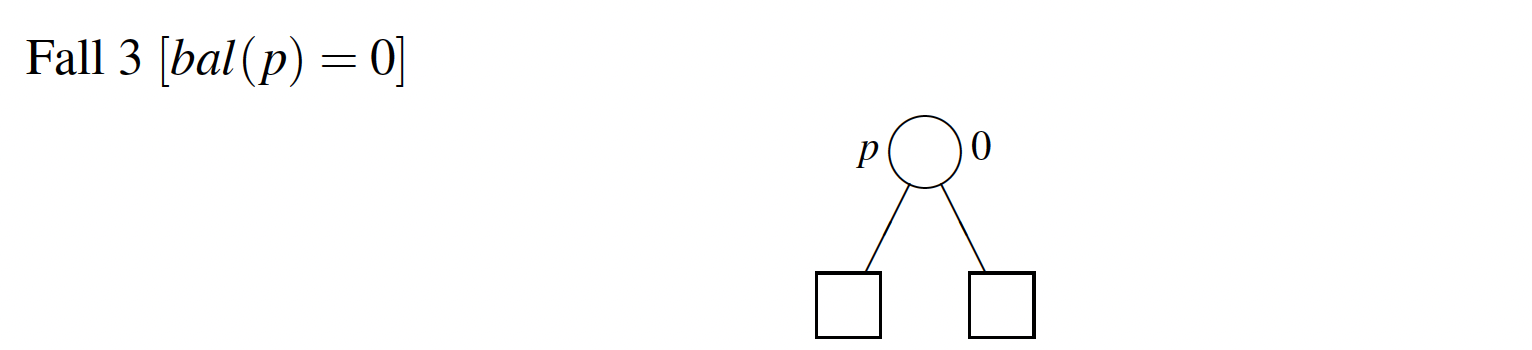
\includegraphics[width=\textwidth]{Pictures/AVL-bal(0).png}
        \caption{$bal(p) = 0$}
        \label{fig: bal(p) = 0}
\end{subfigure}
        
\caption{Veranschaulichung von $bal(p) \in \{-1, 0, +1\}$ und dessen Balancierung}
\label{fig: bal(p) für alle}
\end{figure}

\newpage
\subsubsection{Entfernen}\label{subsection EntfernenAVL}
Wie beim Einfügen in den AVL-Tree gehen wir zuerst so vor wie in natürlichen Suchbäumen. Man sucht den zu entfernenden Schlüssel, findet man diesen nciht, so ist das Entfernen beendet. Falls dies nicht der Fall ist, haben wir drei Fälle der Entfernung. 

\subsubsection*{Fall 1}

Knoten $n$ hat zwei blätter als Kinder. Sei $p$ der Elternknoten von $n \implies $ Anderer Teilbaum hat Höhe $h' =$ 0, 1 oder 2.
\begin{itemize}
    \item $h' = $1: $bal(p)$ anpassen
    \item $h' = $0: $bal(p)$ anpassen. Aufruf von $upout(p)$
    \item $h' = $2: Rebalancieren des Teilbaumes. Aufruf von $upout(p)$
\end{itemize}



\subsubsection*{Fall 2}
Knoten $n$ hat einen inneren Knoten $k$ als Kind
\begin{itemize}
    \item Ersetze $n$ durch $k$ -  $upout(k)$ \ref{fig: upout(p)}
\end{itemize}



\subsubsection*{Fall 3}
Knoten $n$ hat zwei inneren Knoten als Kinder
\begin{itemize}
    \item Ersetze $n$ durch symmetrischen Nachfolger-  $upout(k)$ \ref{fig: upout(p)}
    \item Löschen des symmetrischen Nachfolgers wie in Fall 1 oder 2.
\end{itemize}


\subsubsection*{upout(p)}
Sei $pp$ der Elternknoten von $p$
\begin{itemize}
    \item $p$ linkes Kind von $pp$
        \begin{enumerate}
            \item $bal(pp) = -1 \implies bal(s) \gets 0 \ \textbf{$upout(pp)$}$
            \item $bal(pp) = 0 \implies bal(s) \gets 1 $
            \item $bal(pp) = +1 \implies $ (Vgl. unten \ref{fig: upout(p)})
        \end{enumerate}
    \item $p$ rechtes Kind von $pp$: Symmetrische Fälle unter Veratuschung von -1 und +1
\end{itemize}

\begin{figure}[h!]
\centering
\begin{subfigure}{0.38\textwidth}
    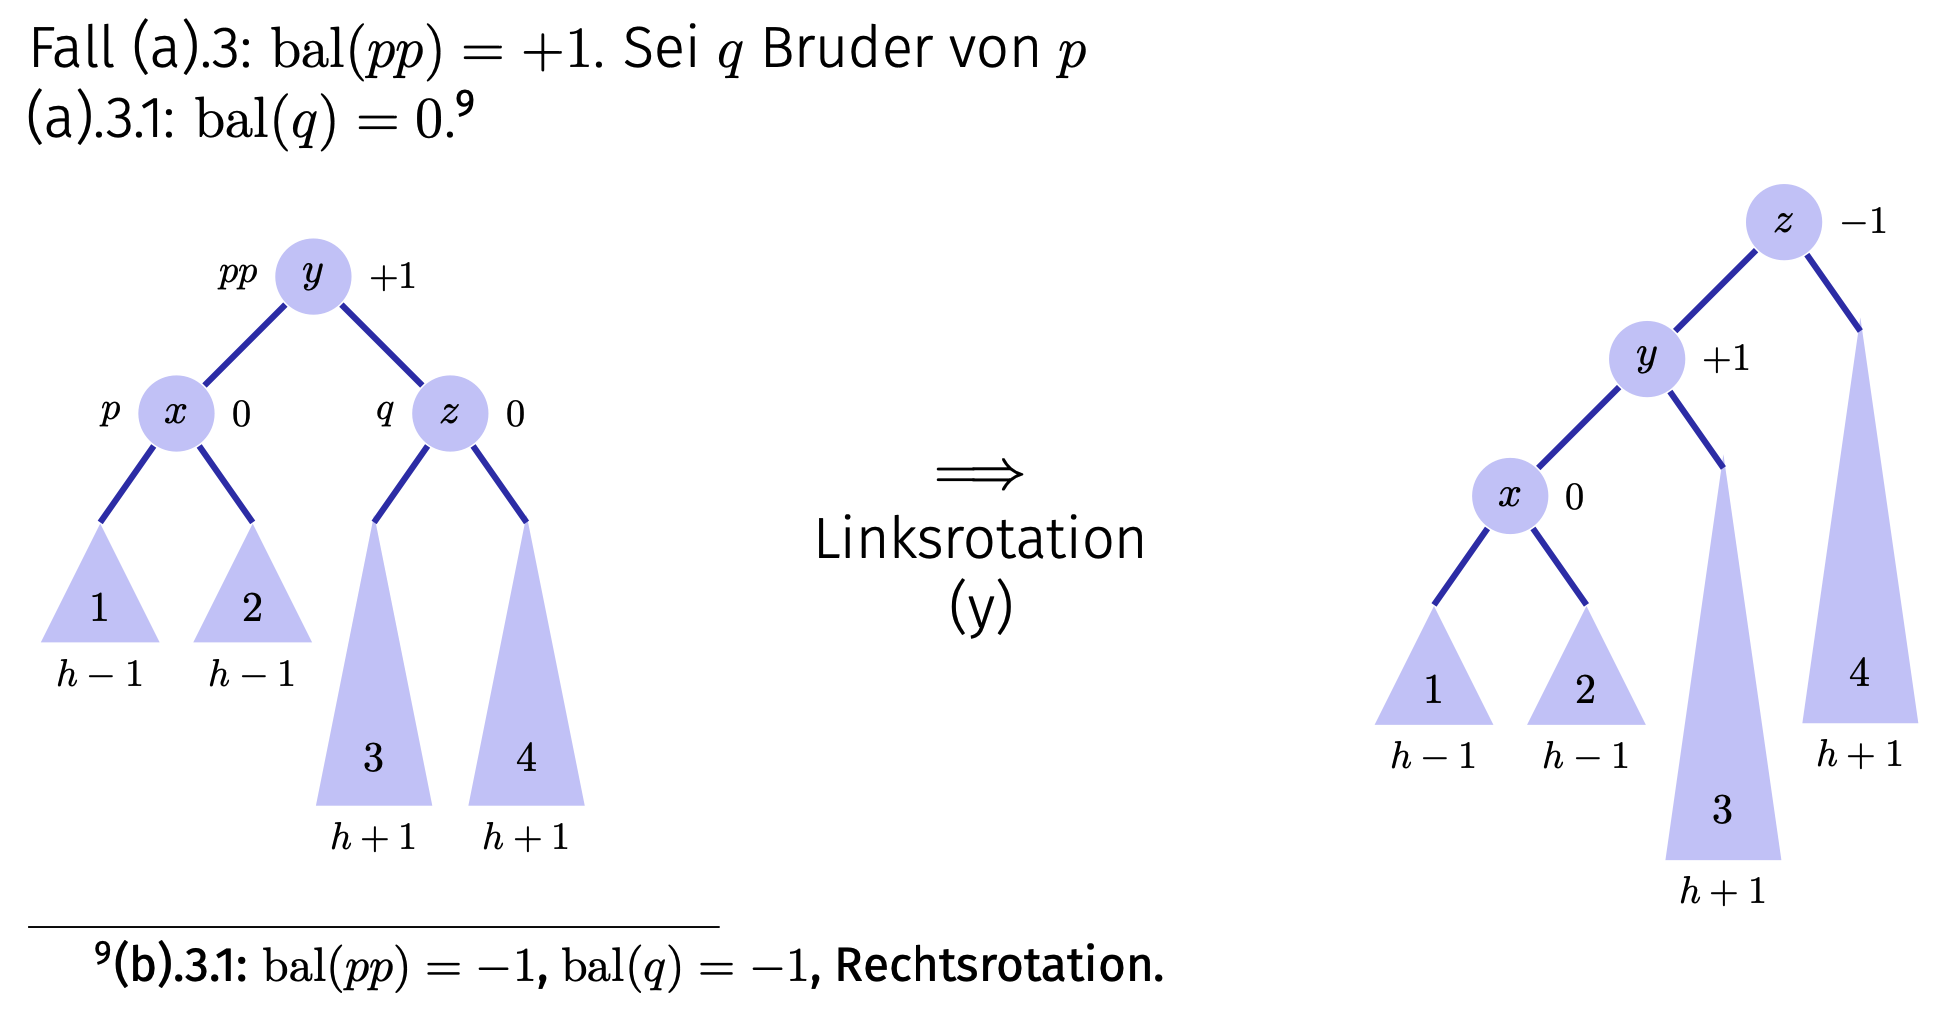
\includegraphics[width=\textwidth]{Pictures/upout1.png}
        \caption{Erster Schritt}
        \label{fig: upout1}
\end{subfigure}
\hfill
\begin{subfigure}{0.38\textwidth}
 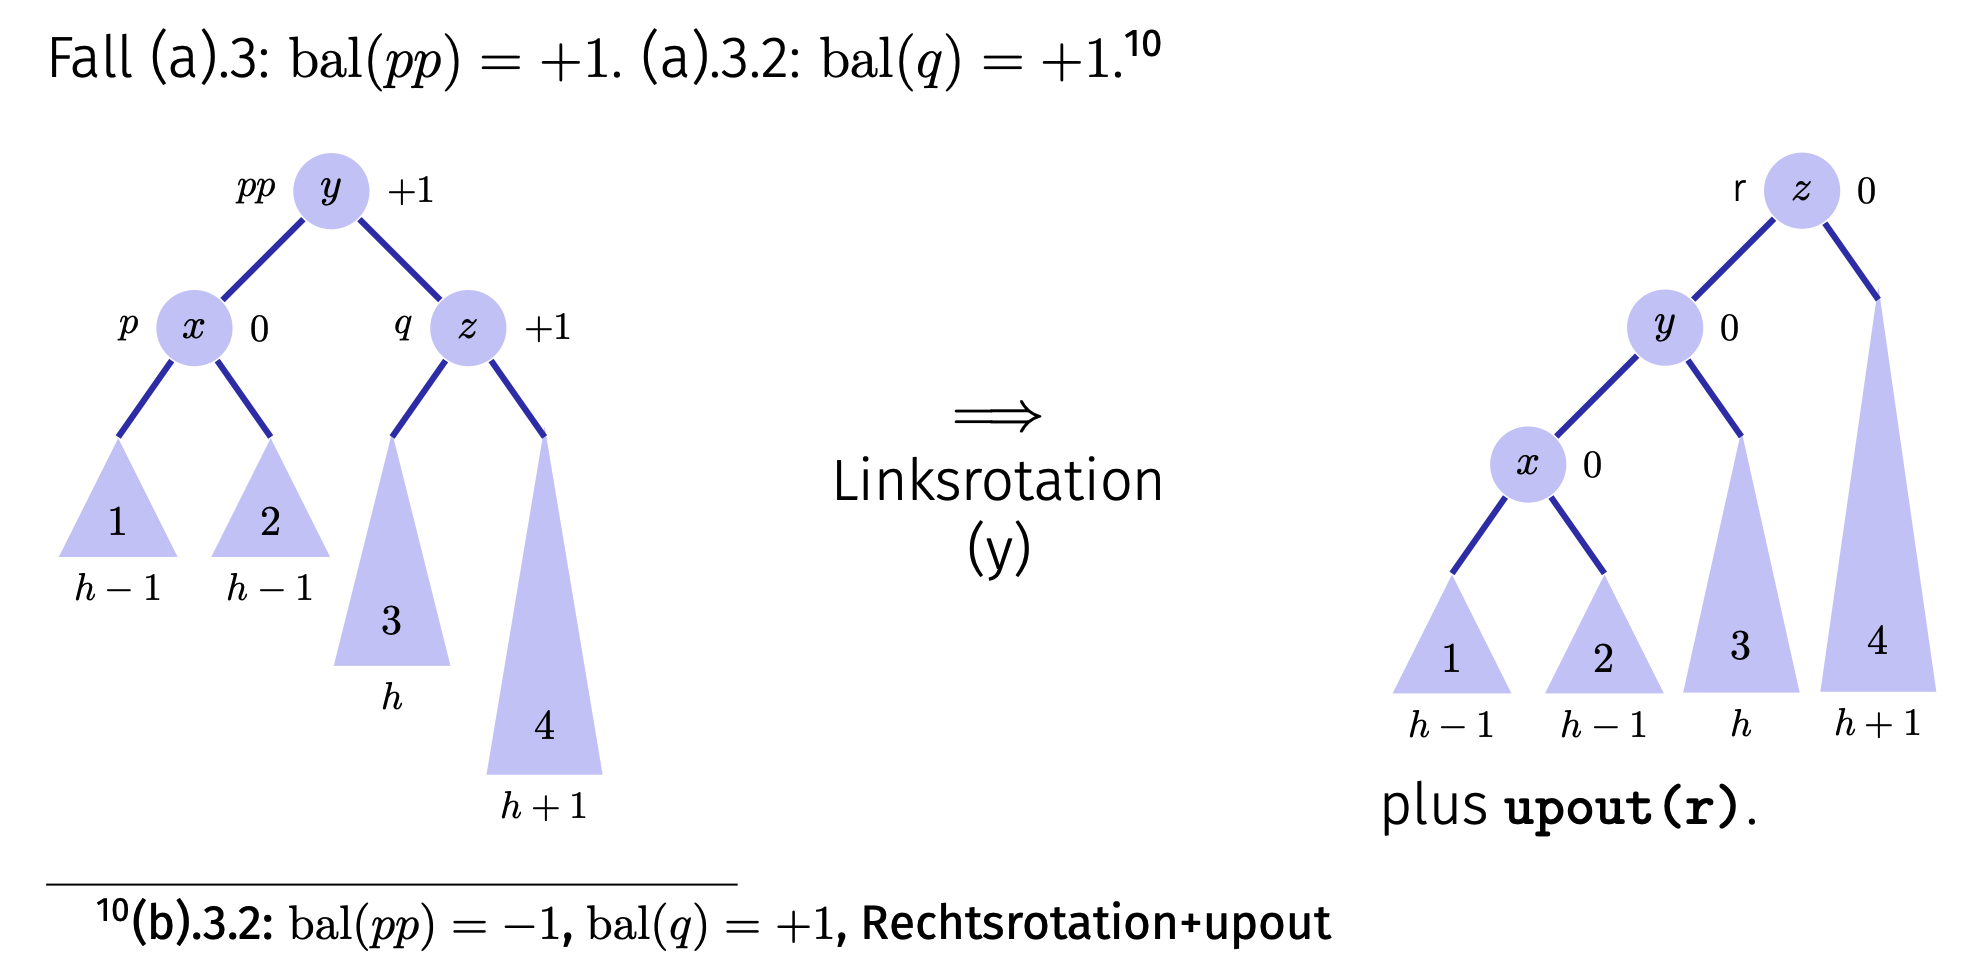
\includegraphics[width=\textwidth]{Pictures/upout2.png}  
 \caption{Zweiter Schritt}
        \label{fig: upout2}
\end{subfigure}

\begin{subfigure}{0.38\textwidth}
 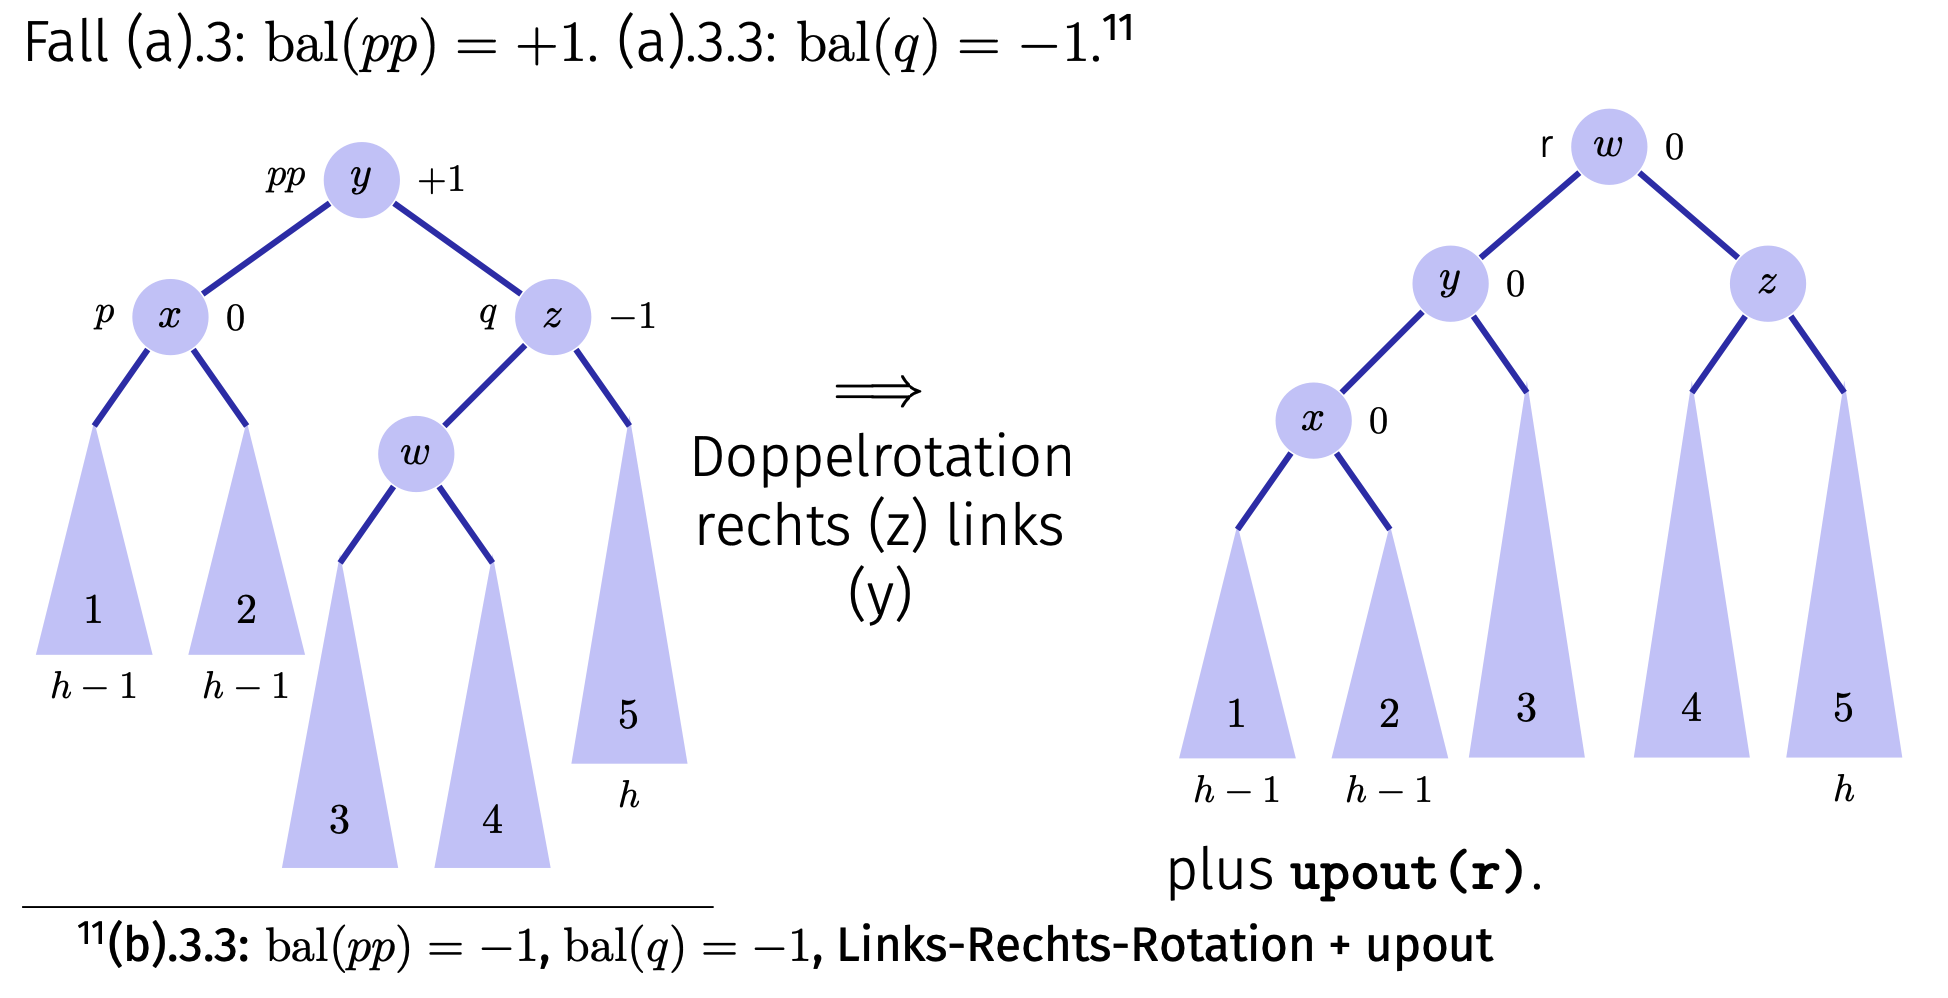
\includegraphics[width=\textwidth]{Pictures/upout3.png}
        \caption{Dritter Schritt}
        \label{fig: upout3}
\end{subfigure}
        
\caption{$upout(p)$, Mit (a) ist der Erste bullet point ($p$ linkes Kind von $pp$) gemeint}
\label{fig: upout(p)}
\end{figure}


\newpage


\subsubsection{Rotationen} \label{Rotationsabschnitt}
In den vorherigen Abschnitten (\ref{subsection EinfügenAVL}, \ref{subsection EntfernenAVL}) haben wir bereits \textbf{Rotationen} gesehen. Wir unterscheiden insgesamt 4 Fälle: LR, RL, LL, RR. \\
LL und RR müssen jeweils nur eine Operation durchführen, wohingegen LR und RL zwei Operationen durchführen müssen. 

\begin{figure}[h]
    \centering
    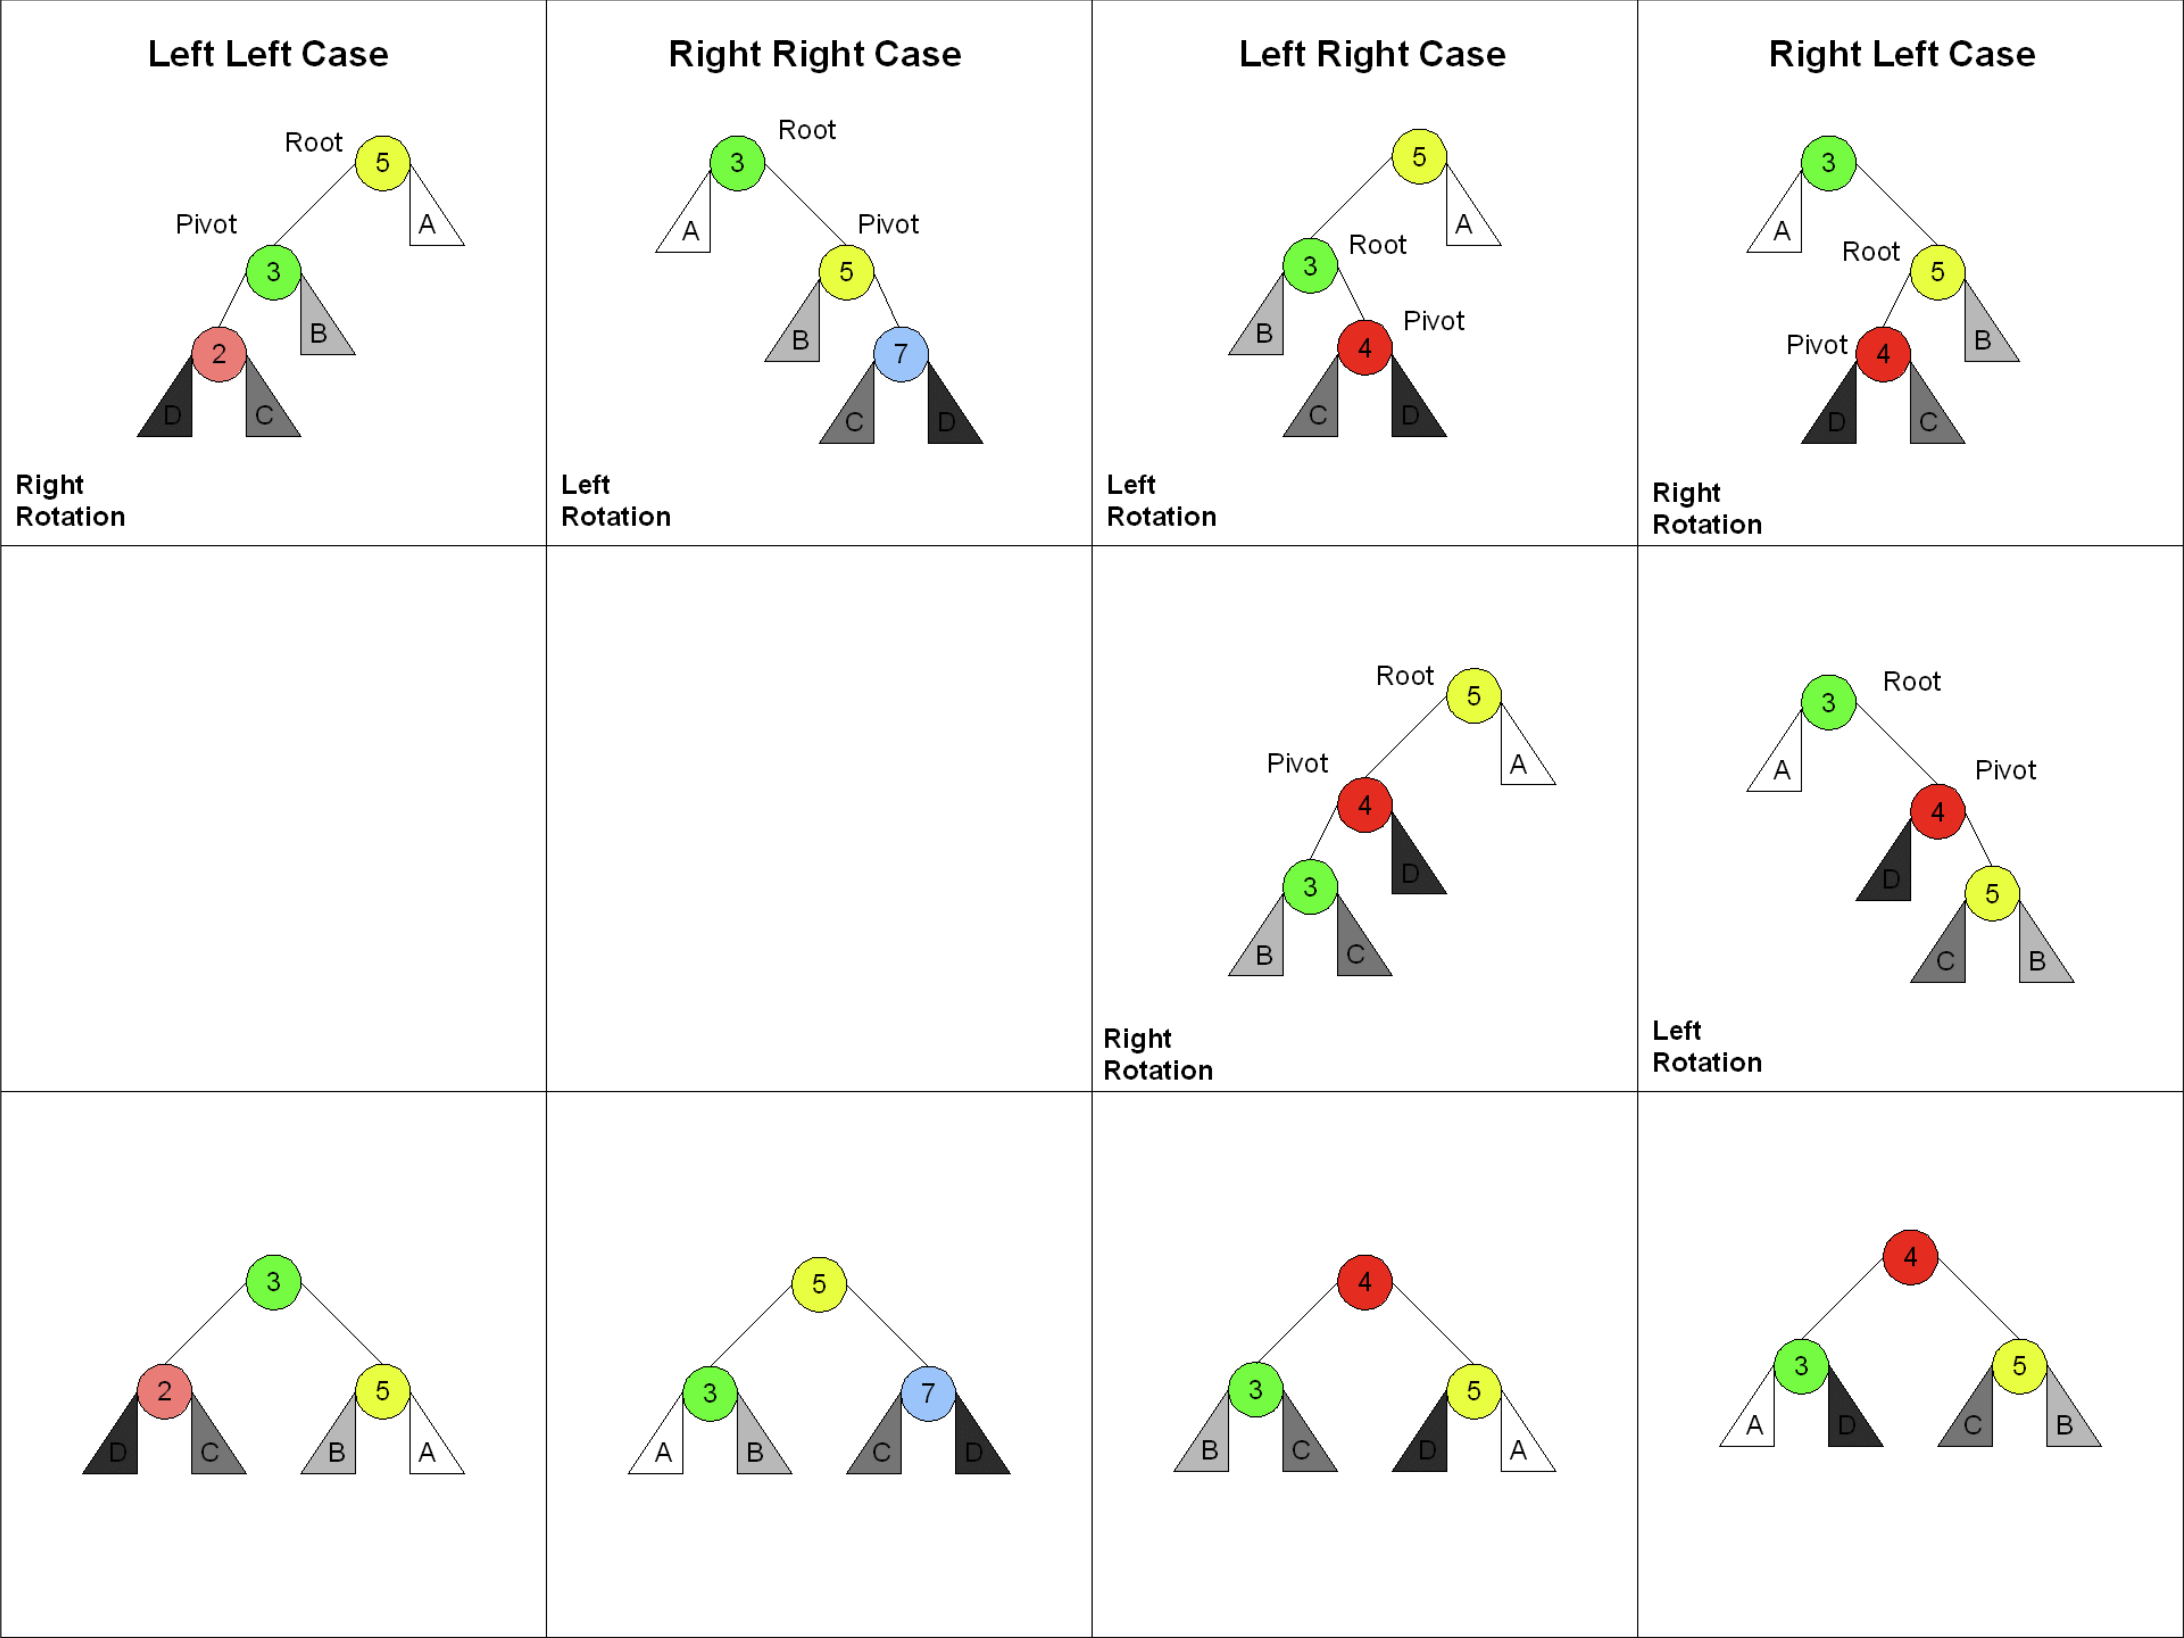
\includegraphics[scale = 0.4]{Pictures/AVL-Rotations.png}
    \caption{Alle Fälle zum AVL-Tree zu balancieren}
    \label{fig:AVL-rotations}
\end{figure}

\subsubsection{Operationen und Komplexität}
    Der Baum braucht genau $\Theta (n)$ Speicher. Er verfügt über die Standartoperationen von Suchen, Einfügen und Entfernen, die eine Komplexität von $\mathcal{O}(\log n)$ haben. 

    \newpage

\subsection{Sortier-Algorithmen}
Zunächst wollen wir das Sortierproblem genauer fixieren: Wir nehmen an, es sei eine
Menge von Sätzen gegeben; jeder Satz besitzt einen Schlüssel. Zwischen Schlüsseln ist
eine Ordnungsrelation „<" oder „$\leq$" erklärt. Außer der Schlüsselkomponente können
Sätze weitere Komponenten als „eigentliche“ Information enthalten.


\subsubsection{Eigenschaften von Sortier-Algorithmen}

\paragraph{Stability} Zwei Objekte mit gleichen Schlüsseln erscheinen in der (sortierten) Ausgabe in der gleichen Reihenfolge, wie sie in der Eingabe erschienen.
\paragraph{In-place} oder in-situ beschreiben jene Algorithmen, die die Eingabe ohne zusätzliche Datenstruktur und damit ohne zusätzlichen Speicherplatz umwandeln. In einigen Fällen ist zusätzlicher Speicherplatz zur Speicherung einiger Variablen zulässig.

\begin{table}[H]
\centering
\caption{Properties of sorting algorithms}
\label{my-label}
~\\
\begin{tabular}{|r|c|c|c|c|c|c|@{}}
  \cline{2-7}
  \multicolumn{1}{c|}{} & \textbf{bubble} & \textbf{insert} & \textbf{select} & \textbf{quick} & \textbf{merge} & \textbf{heap} \\
        \hline
stable  & Yes      & Yes      & No      & No     & Yes     & No    \\
  in-situ & Yes      & Yes      & Yes      & Yes     & No     & Yes   \\
  \hline
\end{tabular}
\end{table}


\subsubsection{Bogo sort}
Bogo sort $\mathcal{O}(n\cdot n!)$ - This is a fairly inefficient sorting algorithm that generates a random permutation until the elements are sorted. An analogy with a deck of card would be to shuffle the deck, then check if it is sorted and loop if it is not. 


\begin{algorithm}
    \caption{Bogo Sort}
    \label{alg:BogoSort}
    \begin{algorithmic}
        \While{$\neg \textsc{isSorted}\left(A\right)$}
        \State $A \gets \textsc{randomPermutation}\left(A\right)$
        \EndWhile
    \end{algorithmic}
\end{algorithm}
This algorithm doesn't have a worst case asymptotic time as it is not guaranteed to terminate within a given time. 

\subsubsection{Stalin-Sort}
The Stalin sort is a sort in which elements that are out of order get removed from a list. For example, [1, 2, 5, 3, 6, 4, 10] becomes [1, 2, 5, 6, 10]. It is said to runs in $\mathcal{O}(n)$ time but if coded that way, the final list may have fewer than the maximum number of elements possible. For example [10, 1, 2, 3, 4] would become [10].

\newpage

    \subsubsection{Bubblesort}\label{Bubblesort}
    Bubblesort $\mathcal{O}(n^2)$ - ist ein Verfahren, welches nach dem Motto \textit{Sortierten durch Einfügen} leben. Bubblesort ist ein Sortierverfahren, das solange zwei jeweils
    benachbarte, nicht in der richtigen Reihenfolge stehende Elemente vertauscht, bis keine Vertauschungen mehr nötig sind.
    Um ein genaueres Verständnis zu erlangen ein Beispiel: \\
    
    \begin{table}[h]
        \centering
        \begin{tabular}{c|c|c|c}
            \textbf{1. (Schritt 6 \& 5)}    & 
            \textbf{2.}    & 
            \textbf{3.}    &
            \textbf{4.}   \\
            
            \hline
            6 5 3 1 8 7 2 4 & 
            \textcolor{red}{3 5} 1 6 7 2 4 8  &
            1 \textcolor{red}{3 5} 6 2 4 7 8 & 
            1 3 \textcolor{red}{2 5} 4 6 7 9 \\
            
            \textcolor{red}  {5 6} 3 1 8 7 2 4 &
            3\textcolor{red} {1 5} 6 7 2 4 8 &
            1 3 \textcolor{red}{5 6} 2 4 7 8 & 
            1 3 2 \textcolor{red}{4 5} 6 7 9 \\
            
            5 \textcolor{red}{3 6} 1 8 7 2 4 &
            3 1 \textcolor{red}{5 6} 7 2 4 8 &
            1 3 5 \textcolor{red}{2 6} 4 7 8 &
            1 3 2 4 \textcolor{red}{5 6} 7 9 \\

            5 3 \textcolor{red}{1 6} 8 7 2 4 & 
            3 1 5 \textcolor{red}{6 7} 2 4 8 &
            1 3 5 2 \textcolor{red}{4 6} 7 8 &
            1 3 2 4 5 \textcolor{red}{6 7} 9 \\

            5 3 1 \textcolor{red}{6 8} 7 2 4 &
            3 1 5 6 \textcolor{red}{2 7} 4 8 &
            1 3 5 2 4 \textcolor{red}{6 7} 8 &
            1 3 2 4 5 6 \textcolor{red}{7 9} \\

            5 3 1 6 \textcolor{red}{7 8} 2 4 &
            3 1 5 6 2 \textcolor{red}{4 7} 8 &
            1 3 5 2 4 6 \textcolor{red}{7 8} &
            \textcolor{red}{1 3} 2 4 5 6 7 9\\

            5 3 1 6 7  \textcolor{red}{2 8} 4 &
            3 1 5 6 2 4  \textcolor{red}{7 8} &
             \textcolor{red}{1 3} 5 2 4 6 7 9 &
            1  \textcolor{red}{2 3} 4 5 6 7 9 \\

            5 3 1 6 7 2 \textcolor{red}{4 8} & 
          \textcolor{red}{1 3} 5 6 2 4 7 8 &
            1 \textcolor{red}{3 5} 2 4 6 7 9 &
            \\
       
        \end{tabular}
        \caption{Tabelle wird von oben nach unten, links nach rechts interpretiert}
        \label{tab:BubblesortTable}
    \end{table}

\begin{algorithm}
    \caption{Bubble sort}
    \label{alg:BubbleSort}
    \begin{algorithmic} 
        \State $swapped \gets \texttt{true}$
        \While{$swapped$}
        \State $swapped \gets \texttt{false}$
        \For {$i \in \left\lbrace 0, \dots, A\texttt{.length}-1 \right\rbrace$}
        \If{$A\left[i\right]>A\left[i+1\right]$}
        \State Swap $A\left[i\right]$ and $A\left[i+1\right]$
        \State $swapped \gets \texttt{true}$
        \EndIf
        \EndFor
        \EndWhile
    \end{algorithmic}
\end{algorithm}

\newpage
 \subsubsection{InsertionSort}\label{Insertionsort}
    InsertionSort $\mathcal{O}(n^2)$ [worst and average case] - ist ein Algorithmus, der der Art und Weise, wie ein Mensch ein Kartenspiel sortiert, sehr ähnlich ist. Er geht so vor, dass er eine Folge von bereits sortierten Elementen behält und immer das nächste Element in der Folge berücksichtigt. Dieses Element wird dann an der richtigen Stelle in der sortierten Folge eingefügt, wobei alle größeren Elemente nach rechts verschoben werden.
    \begin{figure}[h]
        \centering
        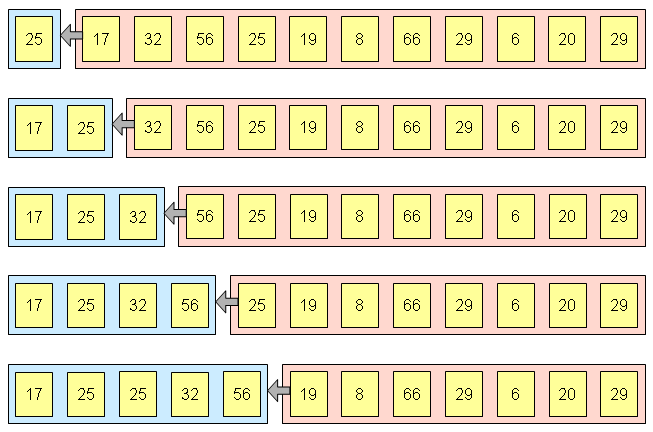
\includegraphics[scale=0.3]{Pictures/insertionsort_version1.png}
        \caption{InsertionSort-Beispiel}
        \label{fig:InsertionSort}
    \end{figure}

\begin{algorithm}
    \caption{Insertion sort}
    \label{alg:InsertionSort}
    \begin{algorithmic} 
        \For {$i \in \left\lbrace 0, \dots, A\texttt{.length} - 1 \right\rbrace$}
        \State $v \gets A\left[i\right]$
        \State $j \gets i-1$
        
        \While{$j\geq 0$ \textbf{and} $A\left[j\right]>v$}
        \State $A\left[j+1\right] \gets A\left[j\right]$
        \State $j\leftarrow j-1$
        \EndWhile
        
        \State $A\left[j+1\right] \gets v$
        \EndFor
    \end{algorithmic}
\end{algorithm}

\newpage
  \subsubsection{SelectionSort}\label{Selectionsort}
   Selection Sort $\Theta(n^2)$ - Dieser Algorithmus behält ebenfalls eine Folge von sortierten Elementen bei und erweitert sie iterativ um das größte der verbleibenden unsortierten Elemente. Dann tauscht er dieses Element mit demjenigen aus, das den sortierten Elementen am nächsten liegt. Dadurch wird das nächste Element ausgewählt, daher der Name.

    \begin{figure}[h]
        \centering
        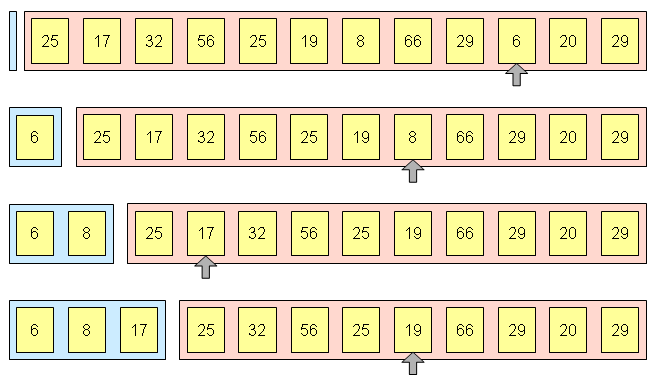
\includegraphics[scale=0.3]{Pictures/selectionsort_idee_version1.png}
        \caption{SelectionSort-Beispiel}
        \label{fig:SelectionSort}
    \end{figure}


    \begin{algorithm}[h]
        \caption{Selection sort}
        \label{alg:SelectionSort}
        \begin{algorithmic} 
          \For{$i \in \left\lbrace 0, A\texttt{.length}-2 \right\rbrace$}
          \State $m, v \gets i, A\left[i\right]$
          \For {$j \in \left\lbrace i+1, \dots, A\texttt{.length} -1\right\rbrace$}
          \If{$A\left[j\right] < v$}
          \State $m, v \gets j, A\left[j\right]$
          \EndIf
          \EndFor
          \If{$m \neq i$}
          \State Swap $A\left[i\right]$ and $A\left[m\right]$
          \EndIf
        
          \EndFor
        \end{algorithmic}
    \end{algorithm}

    \subsubsection*{Complexity}
    Worst case: $\mathcal{O}(n^2)$, Best case: $\mathcal{O}(n^2)$: \\
    $\sum_{i=1}^{n-1} (n-i) = n(n-1)-\sum_{i=1}^{n-1} i = n^2 - n - \frac{n^2-n}{2} = \frac{n^2-n}{2} = \Theta(n^2)$
    
\newpage    

    \subsubsection{Quicksort}\label{Quicksort}
    Quicksort $\mathcal{O}(n\log n)$ - Dieser Algorithmus funktioniert, indem er rekursiv einen Pivot (ein Element, normalerweise an der ersten oder letzten Position im Array) wählt und alle anderen Elemente in Bezug auf diesen aufteilt. Er erstellt zunächst die Mengen $S^-$ und $S^+$, in denen alle Elemente, die kleiner/größer als der Drehpunkt sind, gespeichert werden. Dann ruft es sich selbst rekursiv auf diesen beiden Mengen auf, und nachdem sie sortiert zurückgegeben wurden, fügt es sie einfach zusammen, wobei es den Drehpunkt in der Mitte hinzufügt. Die Rekursion endet im Basisfall, in dem das Array nur ein Element enthält. Es ist zu beachten, dass auch eine In-Place-Implementierung möglich ist, die den Speicher-Overhead reduziert. Dieser Algorithmus hat eine schlechtere obere Schranke für die Operationszeit, wird aber in der Praxis häufig verwendet, da die durchschnittliche Zeit besser ist als bei Merge und Heap Sort. Beachten Sie, dass der $\cdot$-Operator hier Verkettung bedeutet.

    \begin{algorithm}[h]
        \caption{Quicksort}
        \begin{algorithmic}
            \label{alg:Quicksort}
        \Function{QuickSort}{$A$}
        \If{$A\texttt{.length} \leq 1$}
        \State \Return $A$
        \EndIf
        \State Pick pivot $p \gets A[0]$
        \For{$i \in \left\lbrace 1, \dots, A\texttt{.length}-1 \right\rbrace$}
        \If{$A\left[i\right]\leq p$}
        \State $S^-\texttt{.add}\left(A\left[i\right]\right)$
        \Else
        \State $S^+\texttt{.add}\left(A\left[i\right]\right)$
        \EndIf
        \EndFor
        \State $S^+ \gets \textsc{QuickSort}\left(S^+\right)$
        \State $S^- \gets \textsc{QuickSort}\left(S^-\right)$
        \State \Return $S^- \cdot \left\lbrace p\right\rbrace \cdot S^+$
        \EndFunction
        \end{algorithmic}
        \end{algorithm}
        
\newpage
    \subsubsection{Mergesort}\label{Mergesort}
        Mergesort $\mathcal{O}(n \log n)$ - Dieser Algorithmus arbeitet ebenfalls rekursiv. Er teilt die Eingabe in zwei Mengen auf und ruft sich dann selbst rekursiv auf diesen Mengen auf. Nachdem die beiden Mengen sortiert zurückgegeben wurden, führt er sie in linearer Zeit zusammen. Der Name leitet sich von diesem letzten Teil des Algorithmus ab.
        
        \begin{algorithm}[h]
            \caption{Merge sort}
            \label{alg:MergeSort}
            \begin{algorithmic}
              \Function{MergeSort}{$A$}
              \If{$A\texttt{.length} \leq 1$}
              \State \Return $A$
              \EndIf
              \State $n \gets A\texttt{.length}$
              \State $n_1 \gets \frac n2$
              \State $n_2 \gets n-n_1$
              \For{$i \in \left\lbrace 0, \dots, A\texttt{.length} - 1 \right\rbrace$}
              \If{$i < n_1$}
              \State $S^-\texttt{.add}\left(A\left[i\right]\right)$
              \Else
              \State $S^+\texttt{.add}\left(A\left[i\right]\right)$
              \EndIf
              \EndFor
              \State $S^+ \gets \textsc{MergeSort}\left(S^+\right)$
              \State $S^- \gets \textsc{MergeSort}\left(S^-\right)$
              % merge
              \State $i\gets 0$ \Comment{Merge $S^+$ and $S^-$}
              \State $j\gets 0$
              \While{$i<n_1$ \textbf{and} $j<n_2$}
              \If{$S^-\left[i\right]\leq S^+\left[j\right]$}
              \State $R\texttt{.add}\left(S^-\left[i\right]\right)$
              \State $i \gets i+1$
              \Else
              \State $R\texttt{.add}\left(S^+\left[j\right]\right)$
              \State $j \gets j+1$
              \EndIf
              \EndWhile
              \State Concatenate remaining elements to $R$
              \State \Return $R$
              \EndFunction
            \end{algorithmic}
            \end{algorithm}
            
        
\newpage
    \subsubsection{Heapsort}\label{Heapsort}
        Heapsort $\mathcal{O}(n \log n)$ - Dieser Sortieralgorithmus arbeitet, indem er alle Schlüssel in einen Min-Heap einfügt und iterativ das Minimum (die Wurzel) in konstanter Zeit extrahiert und an die Liste der sortierten Knoten anhängt. Er macht dies $n$ Mal; die Gesamtlaufzeit hängt von der Komplexität der Standard-Heap-Operationen ab.
        
        \begin{algorithm}[h]
            \caption{Heap sort}
            \label{alg:HeapSort}
            \begin{algorithmic} 
            \State $H \gets \textsc{CreateMinHeap}\left(\right)$
            \For{$i \in \left\lbrace 0, \dots, A\texttt{.length}-1 \right\rbrace$}
            \State $H\texttt{.insert}\left(A\left[i\right]\right)$
            \EndFor
            \For{$i \in \left\lbrace 0, \dots, A\texttt{.length}-1 \right\rbrace$}
            \State $v \gets H\texttt{.pop}\left(\right)$
            \State $R\texttt{.add}\left(v\right)$
            \EndFor
            \State \Return $R$
            \end{algorithmic}
        \end{algorithm}
        

    \subsubsection{Kosten von Sortieralgorithmen}
    Hier werden die minimalen und maximalen Kosten für einige Sortieralgorithmen auf der Grundlage ihrer Eingabegröße n angegeben, sowie die besondere Art der Eingabe, die zu dieser besonderen Komplexität führt.
    \begin{table}[H]
      \centering
      \footnotesize
      \caption{Best and worst case costs für sortier Algorithmen}
      \label{Sorting 1}
      ~\\
      \hspace{-1.6cm}
      \begin{tabular}{|l | c c | c c | c c | c c |}
        \cline{2-9}
        \multicolumn{1}{c|}{} & \multicolumn{2}{c|}{\textbf{bubblesort}} & \multicolumn{2}{c|}{\textbf{insertion sort}} & \multicolumn{2}{c|}{\textbf{selection sort}} & \multicolumn{2}{c|}{\textbf{quicksort}} \\
        \multicolumn{1}{c|}{}             & best case                & worst case                & best case                  & w.c.                  & best case                  & w.c.                  & best case               & w.c.               \\
        \hline
        \# comparisons  & $\Theta(n)$                  & $\Theta(n^2)$                  & $\Theta(n)$                    & $\Theta(n^2)$                    & $\Theta(n^2)$                    & $\Theta(n^2)$                    & $\Theta(n \log n)$                                  & $\Theta(n^2)$                 \\
        \# permutations & $0$                   & $\Theta(n^2)$                  & $0$                     & $\Theta(n^2)$                    & $0$                     & $\Theta(n)$                    & $\Theta(n)$                   & $\Theta(n \log n)$                 \\
        \hline
        corresponding order             & A                 & B                 & A                   & B & A                   & C                   & C                    & C                 \\
        \hline
      \end{tabular}
      \begin{itemize}
      \item A = already ordered
      \item B = inverse order
      \item C = special order
      \end{itemize}
    
    
    \end{table}
    
     
    \subsubsection{Lower-bound für sortier Algorithmen}
    Jegliche Sortieralgorithmen haben eine worst-case runtime von $\Omega(n \log n)$. Mehr dazu in \textit{Algorithmen und Wahrscheinlichkeiten, ConvexHull}
        
        


%%Chapter 04
ERGÄNZUNGEN MACHEN ZU HEAPSORT, RSP BEISPIELE WIE SICH DIES DURCHSPIELEN LÄSST
\section{GraphenTheorie}
ERGÄNZUNGEN MACHEN ZU HEAPSORT, RSP BEISPIELE WIE SICH DIES DURCHSPIELEN LÄSST
\subsection{Grundlagen}
ERGÄNZUNGEN MACHEN ZU HEAPSORT, RSP BEISPIELE WIE SICH DIES DURCHSPIELEN LÄSST
\subsection{Tiefensuche}
    
\subsection{Breitensuche}
    
\subsection{Zusammenhangskompontente}
    
\subsection{Shortest-path...}
    
\subsubsection{...mit uniformen Kantengewichten}
    
\subsubsection{...mit nicht-negativen Kantengewichten}
    
\subsubsection{...mit allgemeinen Kantengewichten}
    
\subsubsection{...zwischen allen Paaren von Knoten}
    
    
%%Chapter 05
\section{Dynamisches Programmieren}

\subsection{Längste aufsteigende Teilfolge}

\subsection{Längste gemeinsame Teilfolge}

\subsection{Minimale Editierdistanz}

\subsection{Matrixkettenmultiplikation}

\subsection{Subset Sum Problem}

\subsection{Knap Sack Problem}





%%Chapter 06
\section{Sprachunterschiede}





\end{document}
